\documentclass[12pt, a4paper]{article}
\usepackage[a4paper, margin = 2cm]{geometry}
\usepackage[utf8]{inputenc}
\usepackage[T1]{fontenc}
\usepackage{graphicx}
\usepackage{amsmath,amssymb,amsthm,ragged2e}
\usepackage{booktabs}
\usepackage{tabularx}
\usepackage{float}
\linespread{1.5}
\usepackage{hyperref}
\usepackage{authblk}
\usepackage[authoryear]{natbib}
\usepackage{algorithm}
\usepackage{algpseudocode}
\usepackage[toc,page]{appendix}
\usepackage[dvipsnames]{xcolor}
\hypersetup{colorlinks,linkcolor={blue},citecolor={blue},urlcolor={blue}}
\graphicspath{{../../simulation/figures/}{../../application/figures/}}

\newcommand{\jorge}[1]{{\leavevmode\color{red}[#1]}}
\newcommand{\rowan}[1]{{\leavevmode\color{orange}[#1]}}
\newcommand{\yandira}[1]{{\leavevmode\color{teal}[#1]}}
\newcommand{\todo}[1]{{\leavevmode\color{gray}[To write: #1]}}

% Proposed title (to agree with the co-authors)
\title{Covariate-adjusted hot and cold spots of urban pests with eigenvector spatial filtering}
\date{\today}
\author[1,2]{Yandira Cuvero}
\author[3]{Rowan Cherodian}
\author[1]{Jorge Mateu}
\author[2]{Carlos Almeida}
\affil[1]{Department of Mathematics, Universidad Jaume I, Castellón, Spain}
\affil[2]{Department of Mathematics, Escuela Politécnica Nacional, Quito, Ecuador}
\affil[3]{School of Medicine and Population Health, University of Sheffield, UK}

\begin{document}
\maketitle

\begin{abstract}
\todo{abstract, once all sections are written}
\end{abstract}

\section{Introduction}\label{sec1}
\todo{rewrite after the methods are agreed. Plan:
(1) resource allocation for urban pests and the public health motivation (keep from the previous version);
(2) hot-spot detection: local statistics ($G_i^*$, LISA) and risk maps \citep{tamayo2014risk}; reports are not abundance;
(3) gap: hot spots should be defined relative to local characteristics, with error control, and evaluated against benchmarks;
(4) contribution: a covariate-adjusted hot/cold map with ESF, a test before mapping and a permutation band; simulation study with benchmarks; application with exposure, environment and a second species;
(5) outline.}

%%%%%%%%%%%%%%%%%%%%%%%%%%%%%%%%%%%%%%%%%%%%%%%%%%%%%%%%%%%%%%%%%%%%%%%%%%%%%%%%%%%%%%%%%%%
\section{Method}\label{sec:met}
%%%%%%%%%%%%%%%%%%%%%%%%%%%%%%%%%%%%%%%%%%%%%%%%%%%%%%%%%%%%%%%%%%%%%%%%%%%%%%%%%%%%%%%%%%%

\subsection{Setting and definition of a hot spot}\label{sec:setting}

The study region $R$ is partitioned into $n$ cells $c_1,\dots,c_n$. For each cell we observe the number of reported sightings $Y_i$ and a vector of $k$ covariates $z_i$ (local characteristics such as building age or the distance to green areas). Spatial relations between cells are described by a binary, symmetric contiguity matrix $A=(a_{ij})$, with $a_{ij}=1$ when cells $i$ and $j$ share a border or a corner (queen contiguity) and $a_{ii}=0$.

Let $y_i$ be the standardised value of $\log(1+Y_i)$, $Z$ the $n\times k$ matrix of standardised covariates and $X=(\mathbf{1},Z)$. We write
\begin{equation}\label{eq:model}
  y = X\beta + f + \varepsilon ,
\end{equation}
where $\beta$ are the covariate effects, $f=(f_1,\dots,f_n)^\top$ is a spatially structured component and $\varepsilon$ is unstructured noise. The component $f$ collects the variation in sightings that the covariates do not explain and that is shared by neighbouring cells. We define a \emph{hot spot} as a cell with $f_i>0$ and a \emph{cold spot} as a cell with $f_i<0$, in both cases when $f_i$ is larger in absolute value than what spatially unstructured noise would produce. A hot spot is therefore an area with more sightings than its local characteristics predict, and with neighbours that share this excess. This definition depends on the covariates: the same data can show different hot spots under different sets of covariates, and Section~\ref{sec:app} uses this to separate where people report from where the environment predicts more pests.

The procedure has four steps: a test for residual spatial structure, an estimate of $f$ by eigenvector spatial filtering, a permutation band that labels each cell as hot, cold or neutral, and the construction of zones and of a priority list. Algorithm~\ref{alg:hotcold} summarises it.

\subsection{Step 1: test for residual spatial structure}\label{sec:gate}

Let $e=M_X y$ be the residuals of the ordinary least squares (OLS) regression of $y$ on $X$, with $M_X=I-X(X^\top X)^{-1}X^\top$. Moran's $I$ of the residuals,
\begin{equation}\label{eq:moran}
  I = \frac{e^\top A e}{e^\top e},
\end{equation}
is compared with its exact mean and variance under the null hypothesis of no spatial correlation, which for regression residuals depend on $X$ and $A$ only \citep{tg07}. With $T_1=\operatorname{tr}(M_XAM_X)$, $T_2=\operatorname{tr}(M_XAM_XM_XAM_X)$ and $d=n-\operatorname{rank}(X)$,
\begin{equation}\label{eq:moran-moments}
  \operatorname{E}(I)=\frac{T_1}{d}, \qquad
  \operatorname{Var}(I)=\frac{2\,(d\,T_2-T_1^2)}{d^2(d+2)}, \qquad
  z_0=\frac{I-\operatorname{E}(I)}{\sqrt{\operatorname{Var}(I)}} .
\end{equation}
If the one-sided $p$-value of $z_0$ is larger than $\alpha$ (we use $\alpha=0.05$), the procedure stops and every cell is labelled neutral: the covariates explain the spatial pattern of the sightings and there is no evidence of hot or cold spots. Otherwise the procedure continues.

\subsection{Step 2: the spatial component by eigenvector spatial filtering}\label{sec:esf}

Eigenvector spatial filtering (ESF) represents spatial patterns as linear combinations of the eigenvectors of the contiguity matrix \citep{grif2000,grif03,tg07}. Let $A=E\Delta E^\top$ with $E=(e_1,\dots,e_n)$ orthonormal and $\Delta=\operatorname{diag}(\delta_1\ge\dots\ge\delta_n)$. The eigenvector $e_j$ is a map over the cells, and its Moran's $I$ is proportional to $\delta_j$: eigenvectors with large positive eigenvalues are smooth patterns at broad scales, eigenvectors with eigenvalues near zero or negative alternate between neighbouring cells. Hot and cold spots are positively autocorrelated by definition, so we use only the candidate set
\begin{equation}\label{eq:candidates}
  \mathcal{C}=\{\,j:\ \delta_j\ge c\,\delta_1\,\}, \qquad c=0.25,
\end{equation}
the threshold suggested by \citet{grif03}. On a regular queen grid this keeps about one fifth of the eigenvectors. With $E_{\mathcal{C}}$ the matrix of candidate eigenvectors, model~\eqref{eq:model} becomes
\begin{equation}\label{eq:esf}
  y = X\beta + E_{\mathcal{C}}\gamma + \varepsilon ,
\end{equation}
and we estimate it by ridge regression \citep{hoerl1970ridge}, penalising the eigenvector coefficients but not the covariate effects:
\begin{equation}\label{eq:ridge}
  (\hat\beta,\hat\gamma) = \arg\min_{\beta,\gamma}\ \frac{1}{2n}\,\lVert y-X\beta-E_{\mathcal{C}}\gamma\rVert_2^2 + \frac{\lambda}{2}\,\lVert\gamma\rVert_2^2 ,
  \qquad
  \hat\gamma=\bigl(E_{\mathcal{C}}^\top M_X E_{\mathcal{C}}+n\lambda I\bigr)^{-1}E_{\mathcal{C}}^\top M_X\, y .
\end{equation}
The penalty $\lambda$ is chosen by ten-fold cross-validation (the value with the smallest cross-validated error), and the model is fitted with the \texttt{glmnet} package \citep{friedman2010regularization}. The estimated spatial component is
\begin{equation}\label{eq:fhat}
  \hat f = E_{\mathcal{C}}\hat\gamma - \overline{E_{\mathcal{C}}\hat\gamma}\,\mathbf{1} ,
\end{equation}
centred because the leading eigenvector of a connected graph is nearly constant and therefore almost collinear with the intercept. When the covariates are close to orthogonal to the candidate eigenvectors, $E_{\mathcal{C}}^\top M_X E_{\mathcal{C}}\approx I$ and ridge shrinks all coefficients by the same factor, so that $\hat f$ is, up to a scale, the projection of the residuals $e$ on the smooth patterns in $\mathcal{C}$. In this sense $\hat f$ is a smoothed residual map, with the amount of smoothing set by the candidate set and adapted to the covariates through $M_X$.

\subsection{Step 3: hot, cold and neutral cells}\label{sec:band}

To decide which values of $\hat f_i$ are larger than noise, we compare them with their distribution when the residuals carry no spatial structure. Following \citet{freedman1983nonstochastic}, for $b=1,\dots,B$ we permute the OLS residuals, $y^{(b)}=X\hat\beta_{\mathrm{OLS}}+\Pi_b e$, with $\Pi_b$ a random permutation matrix, and refit~\eqref{eq:ridge} with the same candidate set and the same $\lambda$, which gives $\hat f^{(b)}$. For each cell let $q_i^{\,\mathrm{lo}}$ and $q_i^{\,\mathrm{hi}}$ be the 5\% and 95\% quantiles of $\hat f_i^{(1)},\dots,\hat f_i^{(B)}$. Cell $i$ is labelled
\begin{equation}\label{eq:labels}
  \text{hot if } \hat f_i>q_i^{\,\mathrm{hi}}, \qquad
  \text{cold if } \hat f_i<q_i^{\,\mathrm{lo}}, \qquad
  \text{neutral otherwise.}
\end{equation}
The band is pointwise: under the null each cell has a 5\% chance of being labelled hot. The test of Step~1 controls the map as a whole, because the band is only computed when the residuals show spatial structure. We use $B=999$ in the application; in the simulation study we use $B=200$ on the $20\times20$ grid and $B=100$ on the $40\times40$ grid to limit computing time.

\subsection{Step 4: zones and priority list}\label{sec:rank}

Hot (cold) zones are the connected components of the hot (cold) cells in the graph of $A$. When resources are limited to $m$ cells, cells are ranked by their estimated excess: first the hot cells by decreasing $\hat f_i$, then the remaining cells by decreasing $\hat f_i$. Since $y$ is the standardised logarithm of the counts, $\hat f_i$ is measured in standard deviations of $\log(1+Y)$: a value of $0.5$ means that the cell and its neighbourhood have about half a standard deviation more log sightings than the covariates predict.

\begin{algorithm}[ht]
\caption{Covariate-adjusted hot and cold spots}\label{alg:hotcold}
\begin{algorithmic}[1]
\State \textbf{Input:} counts $Y$, covariates $Z$, contiguity matrix $A$; level $\alpha$, threshold $c$, permutations $B$, budget $m$.
\State $y\gets$ standardised $\log(1+Y)$; $X\gets(\mathbf{1},Z)$ with $Z$ standardised; $e\gets M_Xy$.
\State Compute $z_0$ from~\eqref{eq:moran}--\eqref{eq:moran-moments}. \textbf{If} its $p$-value $>\alpha$, label all cells neutral and \textbf{stop}.
\State $A=E\Delta E^\top$; $\mathcal{C}\gets\{j:\delta_j\ge c\,\delta_1\}$.
\State Choose $\lambda$ by ten-fold cross-validation; fit~\eqref{eq:ridge}; $\hat f\gets$~\eqref{eq:fhat}.
\For{$b=1,\dots,B$}
  \State $y^{(b)}\gets X\hat\beta_{\mathrm{OLS}}+\Pi_be$; refit~\eqref{eq:ridge} with the same $\mathcal{C}$ and $\lambda$; store $\hat f^{(b)}$.
\EndFor
\State Label each cell hot, cold or neutral with~\eqref{eq:labels}.
\State Hot (cold) zones $\gets$ connected components of hot (cold) cells in $A$.
\State Priority list $\gets$ hot cells by decreasing $\hat f_i$, then the other cells by decreasing $\hat f_i$; return the first $m$.
\end{algorithmic}
\end{algorithm}

\subsection{Rationale for each step}\label{sec:rationale}

Each choice above was compared with alternatives in the simulation study of Section~\ref{sec:sim}. We summarise the reasons here.

\paragraph{Logarithm of the counts.} Counts of sightings are skewed and their variance grows with the mean, so a few cells with many reports dominate a model for the raw counts. On the log scale, the test of Step~1 correctly finds no spatial structure when the pattern is fully explained by a covariate; on the raw scale it does not.

\paragraph{Covariate adjustment.} Without covariates, a hot spot is simply an area with many sightings, and areas where the environment favours the pest are flagged even when nothing else is going on. In the simulation study, ranking cells by their counts (or applying Getis-Ord $G_i^*$ and local Moran's $I$ to the counts) placed most of the selected cells in an area driven by a covariate: the share of the top 5\% of cells inside a true cluster was at most 0.32, and close to zero with weak clusters.

\paragraph{Test before mapping.} Local statistics label some cells as hot even when there is no clustering at all: at the 5\% level, about one cell in twenty. Testing the residuals first removes most of these false hot cells: in the simulation study, $G_i^*$ labelled 4--6\% of the map hot when there were no clusters, and 0.2--1.9\% when it was preceded by the test (Section~\ref{sec:sim}). The same test can be placed in front of any local statistic, and we do so for the benchmarks.

\paragraph{Eigenvector spatial filtering.} ESF estimates the spatial component inside a regression, so the covariates are adjusted for in the same model, and it represents patterns at several scales at once. Local statistics such as $G_i^*$ average each cell with a fixed neighbourhood. In the simulation study this difference matters when clusters of different sizes coexist: ESF finds the smaller clusters more often.

\paragraph{Smooth candidates.} Eigenvectors with small or negative eigenvalues describe patterns that alternate between neighbours and fit cell-level noise. Restricting the candidates to~\eqref{eq:candidates} improved the precision of the top-ranked cells mainly where it was low: with weak clusters and on the finer grid it roughly doubled (for example from 0.17 to 0.36 with cross-validated penalties), with little change elsewhere.

\paragraph{Ridge with cross-validation.} The Moran's $I$ Lasso of \citet{barde2023moran} sets the penalty to $\lambda=|z_0|^{-2}$, a choice with good properties for estimating $\beta$ \citep{barde2024moran}. For mapping $f$ it ties the amount of smoothing to the strength of the Moran signal: with weak clusters ($|z_0|\approx3$) the penalty is large and often no eigenvector is selected, so $\hat f=0$; with strong clusters ($|z_0|>10$) it is so small that almost all eigenvectors enter and $\hat f$ follows the noise. Cross-validation adapts the penalty to the data, and ridge keeps all smooth candidates instead of selecting a few, which avoids the empty selections. Among the eight penalty rules we compared, cross-validation with smooth candidates gave the most stable precision across scenarios, and replacing the Lasso by ridge improved it further with weak clusters (from 0.52 to 0.67 on the $20\times20$ grid). Our aim is to map $f$, not to select eigenvectors consistently, so the theoretical reservations about cross-validation for variable selection \citep{clc21} do not apply here. The labels and rankings were also insensitive to the cross-validation design (random or spatial blocks), which is consistent with the near-uniform shrinkage described after~\eqref{eq:fhat}.

\paragraph{Permutation band.} The distribution of $\hat f_i$ under no spatial structure depends on the covariates, the candidate set and the penalty, and has no simple closed form. Permuting the residuals reproduces the whole estimation in each replicate, so the band accounts for the smoothing that ESF itself introduces. A band for the maximum of $\hat f$ over the map, which would control the chance of any false hot cell, labelled almost no cells in our simulations and was not retained.

\paragraph{What the procedure does not do.} An earlier version of this work reconstructed a sparser spatial graph from the selected eigenvectors, iterated the selection on that graph, and ranked cells by their centrality in it. Appendix~\ref{app:reconstruction} shows that the reconstruction does not recover the graph through which the process spreads, that iterating does not improve the ranking, and that centrality in the reconstructed graph does not distinguish hot from cold areas. The one-pass procedure above replaces it.

%%%%%%%%%%%%%%%%%%%%%%%%%%%%%%%%%%%%%%%%%%%%%%%%%%%%%%%%%%%%%%%%%%%%%%%%%%%%%%%%%%%%%%%%%%%
\section{Simulation study}\label{sec:sim}
%%%%%%%%%%%%%%%%%%%%%%%%%%%%%%%%%%%%%%%%%%%%%%%%%%%%%%%%%%%%%%%%%%%%%%%%%%%%%%%%%%%%%%%%%%%

In this section we test procedure in Algorithm~\ref{alg:hotcold}, identify its characteristics, properties, and also compare it  with standard hot-spot methods on data where the true hot and cold areas are known. All code is available in the repository of the \texttt{hotcoldESF} package, \url{https://github.com/yandiracuvero/hotcoldESF}, archived on Zenodo \citep{hotcoldesf2026}. 
%, and to check the choices of Section~\ref{sec:rationale}. 

\subsection{Design}\label{sec:sim-design}

%\paragraph{Point patterns.}
 Points are generated in the square window $[0,1000]^2$. Every pattern contains three components:
\begin{itemize}
  \item 2000 points distributed uniformly (background);
  \item 3000 points whose intensity follows an environmental covariate: a Gaussian bump $b(u)=\exp\{-\lVert u-u_0\rVert^2/(2\cdot150^2)\}$ centred at a random location $u_0$ away from the clusters, with points accepted with probability $\exp\{3(b(u)-1)\}$;
  \item clusters, generated as a modified Thomas process: each cluster has a centre and a fixed number of points distributed uniformly within a disc (or an ellipse) around it.
\end{itemize}
The covariate area is part of the explained variation: the model receives the covariate $b$ evaluated at the centre of each cell, together with an irrelevant covariate drawn from a standard normal distribution. A method that adjusts for covariates should not label the covariate area as hot.

%\paragraph{Scenarios.} 
Table~\ref{tab:scenarios} lists the scenarios concidered. Scenarios B, L, E, M and S vary the size, shape and number of the clusters; K adds a true cold area, where only a fraction of the points is kept; U has the same data as B but the model does not receive the covariate, to show the effect of a missing covariate; C and N contain no clusters. Every scenario except C and N has a weak and a strong clustering version.

\begin{table}[ht]
\centering
\caption{Simulation scenarios. All patterns also contain 2000 uniform points and 3000 points that follow the covariate; the window is $1000\times1000$.}\label{tab:scenarios}
\small
\begin{tabularx}{\textwidth}{l>{\raggedright\arraybackslash}X>{\raggedright\arraybackslash}X>{\raggedright\arraybackslash}p{3.2cm}}
\toprule
Scenario & Clusters & Points per cluster (weak / strong) & Purpose \\
\midrule
B & 3 discs, radius 100 & 50 / 200 & compact clusters \\
L & 2 discs, radius 200 & 200 / 600 & large, diffuse clusters \\
E & 3 ellipses, semi-axes $300\times33$ & 100 / 300 & elongated clusters \\
M & 3 discs, radii 50, 100, 200 & same intensity: 24, 94, 377 / 50, 200, 800 & clusters of different sizes \\
S & 8 discs, radius 40 & 15 / 40 & many small clusters \\
K & as B (200 points) & cold disc of radius 150 keeps 50\% / 20\% & a true cold area \\
U & as B & 50 / 200; covariate not given to the model & missing covariate \\
C & none & -- & covariate area only \\
N & none & 3000 uniform points, no covariate area & complete spatial randomness \\
\bottomrule
\end{tabularx}
\end{table}

%\paragraph{Grids.} 
Points are counted on a $20\times20$ grid (cell side 50) and on a $40\times40$ grid (cell side 25), with queen contiguity. We generate 100 datasets per setting on the $20\times20$ grid and 50 on the $40\times40$ grid, 2400 datasets in total. The permutation band uses $B=999$ permutations on both grids, as in the application.

%\paragraph{Methods.} 
The proposed procedure (Algorithm~\ref{alg:hotcold}, denoted ESF) is compared with:
\begin{itemize}
  \item Getis-Ord $G_i^*$ \citep{getis1992analysis,ord1995local} on the residuals $u$ of $\log(1+w)$ on the covariates, with binary weights including the cell itself; a cell is hot if $G_i^*>1.645$ and cold if $G_i^*<-1.645$. We consider three versions: alone, preceded by the test of Step~1, and preceded by the test with a false discovery rate correction \citep{benjamini1995controlling};
  \item local Moran's $I$ (LISA) \citep{anselin1995local} on the same residuals, with conditional permutation $p$-values (999 permutations) and preceded by the test; a cell is hot if it is high--high with $p<0.05$, cold if low--low with $p<0.05$;
  \item two rankings without spatial smoothing: the cells with the largest residuals $u$ (top residuals) and the cells with the largest counts (top counts).
\end{itemize}
The $G_i^*$ ranking orders cells by $G_i^*$, and the LISA ranking orders high--high cells by their local $I$.





\subsection{Choices within the procedure}\label{sec:sim-choices}

The choices listed below rest on three sources of evidence. Choices~\ref{ch:log}, \ref{ch:cand}, \ref{ch:ridge} and~\ref{ch:band} were made with preliminary experiments, run before the main study on scenarios A (three clusters of 500 points and 2000 uniform points, no covariate area), B, C and N and on the same two grids (and a $10\times10$ grid for choice~\ref{ch:log}). Choices~\ref{ch:cov}, \ref{ch:test} and~\ref{ch:esf} are supported by the main study, whose results are reported in Section~\ref{sec:sim-results}; for choice~\ref{ch:cov}, the preliminary experiments also applied $G_i^*$ and local Moran's $I$ to the counts. Choice~\ref{ch:lin} comes from a further analysis of 900 datasets of the main study (scenarios B, S and C), refitted with a natural spline for each covariate. The scripts and full results are in the repository.

%\subsection{Rationale for each step}\label{sec:rationale}
%Each choice above was compared with alternatives in the simulation study of Section~\ref{sec:sim}. We summarise the reasons here.

Each item below refers to the line of Algorithm~\ref{alg:hotcold} and the step of Section~\ref{sec:met} that it justifies.

\begin{enumerate}

\item\label{ch:log} \textbf{Logarithm of the counts} (Algorithm~\ref{alg:hotcold}, line~\ref{alg:l-data}: $y\gets$ standardised $\log(1+w)$; Step~1).
Counts of sightings are skewed and their variance grows with the mean, so a few cells with many reports dominate a model for the raw counts. On the log scale, the test of Step~1 correctly finds no spatial structure when the pattern is fully explained by a covariate; on the raw scale it does not.

\item\label{ch:cov} \textbf{Covariate adjustment} (line~\ref{alg:l-data}: $X\gets(\mathbf{1},Z)$ and $u\gets M_Xy$; Step~1).
Without covariates, a hot spot is simply an area with many sightings, and areas where the environment favours the pest are flagged even when nothing else is going on. In the simulation study, ranking cells by their counts (or applying Getis-Ord $G_i^*$ and local Moran's $I$ to the counts) placed most of the selected cells in an area driven by a covariate: the share of the top 5\% of cells inside a true cluster was at most 0.32, and close to zero with weak clusters.

\item\label{ch:lin} \textbf{Linear covariate terms} (line~\ref{alg:l-data}: the columns of $X$; Step~1).
A natural spline with 2 to 4 degrees of freedom for each covariate reduced the false rejections of the test in scenario C from 19--32\% to 4--6\%, but also reduced the rejections with weak small clusters (S) from 64--76\% to 28--44\%: a flexible function of a smooth covariate absorbs part of the cluster signal \citep{hodges2010adding}. We keep linear covariate terms and report the spline version as a sensitivity analysis.

\item\label{ch:test} \textbf{Test before mapping} (line~\ref{alg:l-test}; Step~1).
Local statistics label some cells as hot even when there is no clustering at all: at the 5\% level, about one cell in twenty. Testing the residuals first removes most of these false hot cells: in the simulation study, $G_i^*$ labelled 4.0--5.6\% of the map hot when there were no clusters, and 0.2--1.9\% when it was preceded by the test (Table~\ref{tab:sim-labels}), without any change in its ranking. %The same test can be placed in front of any local statistic, and we do so for the benchmarks.

The test does not depend on how the cells are labelled afterwards, so it can be used as a
first step for any local statistic. In the simulation study we also apply it to the
benchmarks ($G_i^*$ and local Moran's $I$), so that differences between methods in the
number of false hot cells come from the local statistic and not from the test.

\item\label{ch:esf} \textbf{Eigenvector spatial filtering} (lines~\ref{alg:l-cand}--\ref{alg:l-fit}; Step~2).
ESF estimates the spatial component inside a regression, so the covariates are adjusted for in the same model, and it represents patterns at several scales at once. Local statistics such as $G_i^*$ average each cell with a fixed neighbourhood. In the simulation study this difference matters when clusters of different sizes coexist: ESF finds the smaller clusters more often.

\item\label{ch:cand} \textbf{Smooth candidates} (line~\ref{alg:l-cand}: $\mathcal{C}\gets\{j:\delta_j\ge c\,\delta_1\}$; Step~2, equation~\eqref{eq:candidates}).
Eigenvectors with small or negative eigenvalues describe patterns that alternate between neighbours and fit cell-level noise. Restricting the candidates to~\eqref{eq:candidates} improved the precision of the top-ranked cells mainly where it was low: with weak clusters and on the finer grid it roughly doubled (for example from 0.17 to 0.36 with cross-validated penalties), with little change elsewhere.

\item\label{ch:ridge} \textbf{Ridge with a cross-validated penalty} (line~\ref{alg:l-fit}: choice of $\lambda$ and of the estimator; Step~2, equation~\eqref{eq:ridge}).
We compared eight ways to choose the penalty (the Moran's $I$ Lasso rule $|z_0|^{-a}$ with $a=1,2,3,4$; cross-validation with the smallest error and with the one-standard-error rule; BIC; and the largest penalty whose residuals pass the Moran test), each with all eigenvectors or with the smooth candidates~\eqref{eq:candidates}. The rule $|z_0|^{-2}$ of the Moran's $I$ Lasso \citep{barde2023moran} has good properties for estimating $\beta$ \citep{barde2024moran}, but for mapping $f$ it ties the amount of smoothing to the strength of the Moran signal: with weak clusters ($|z_0|\approx3$) the penalty is large and often no eigenvector is selected, so $\hat f=0$; with strong clusters ($|z_0|>10$) it is so small that almost all eigenvectors enter and $\hat f$ follows the noise. With this rule and all eigenvectors, the precision of the top 5\% with weak clusters was 0.19 ($20\times20$) and 0.11 ($40\times40$): the Lasso selected no eigenvector in 6 of 17 datasets with residual structure. Cross-validation with smooth candidates raised these values to 0.52 and 0.36 while keeping 0.98--1.00 with strong clusters, and replacing the Lasso by ridge, which keeps all smooth candidates instead of selecting a few, raised them further to 0.67 and 0.47. Our aim is to map $f$, not to select eigenvectors consistently, so the theoretical reservations about cross-validation for variable selection \citep{clc21} do not apply here. Spatial (block) folds for the cross-validation did not change the results, which is consistent with the near-uniform shrinkage described after~\eqref{eq:fhat}. Figure~\ref{fig:penalty} summarises the comparison: rules that penalise little ($|z_0|^{-3}$, $|z_0|^{-4}$) do well with weak clusters but lose precision with strong ones, rules that penalise more ($|z_0|^{-1}$, the one-standard-error rule, BIC) fail with weak clusters, and cross-validation with smooth candidates is the only Lasso rule that does well in both; ridge improves on it with weak clusters.

\begin{figure}[ht]
\centering
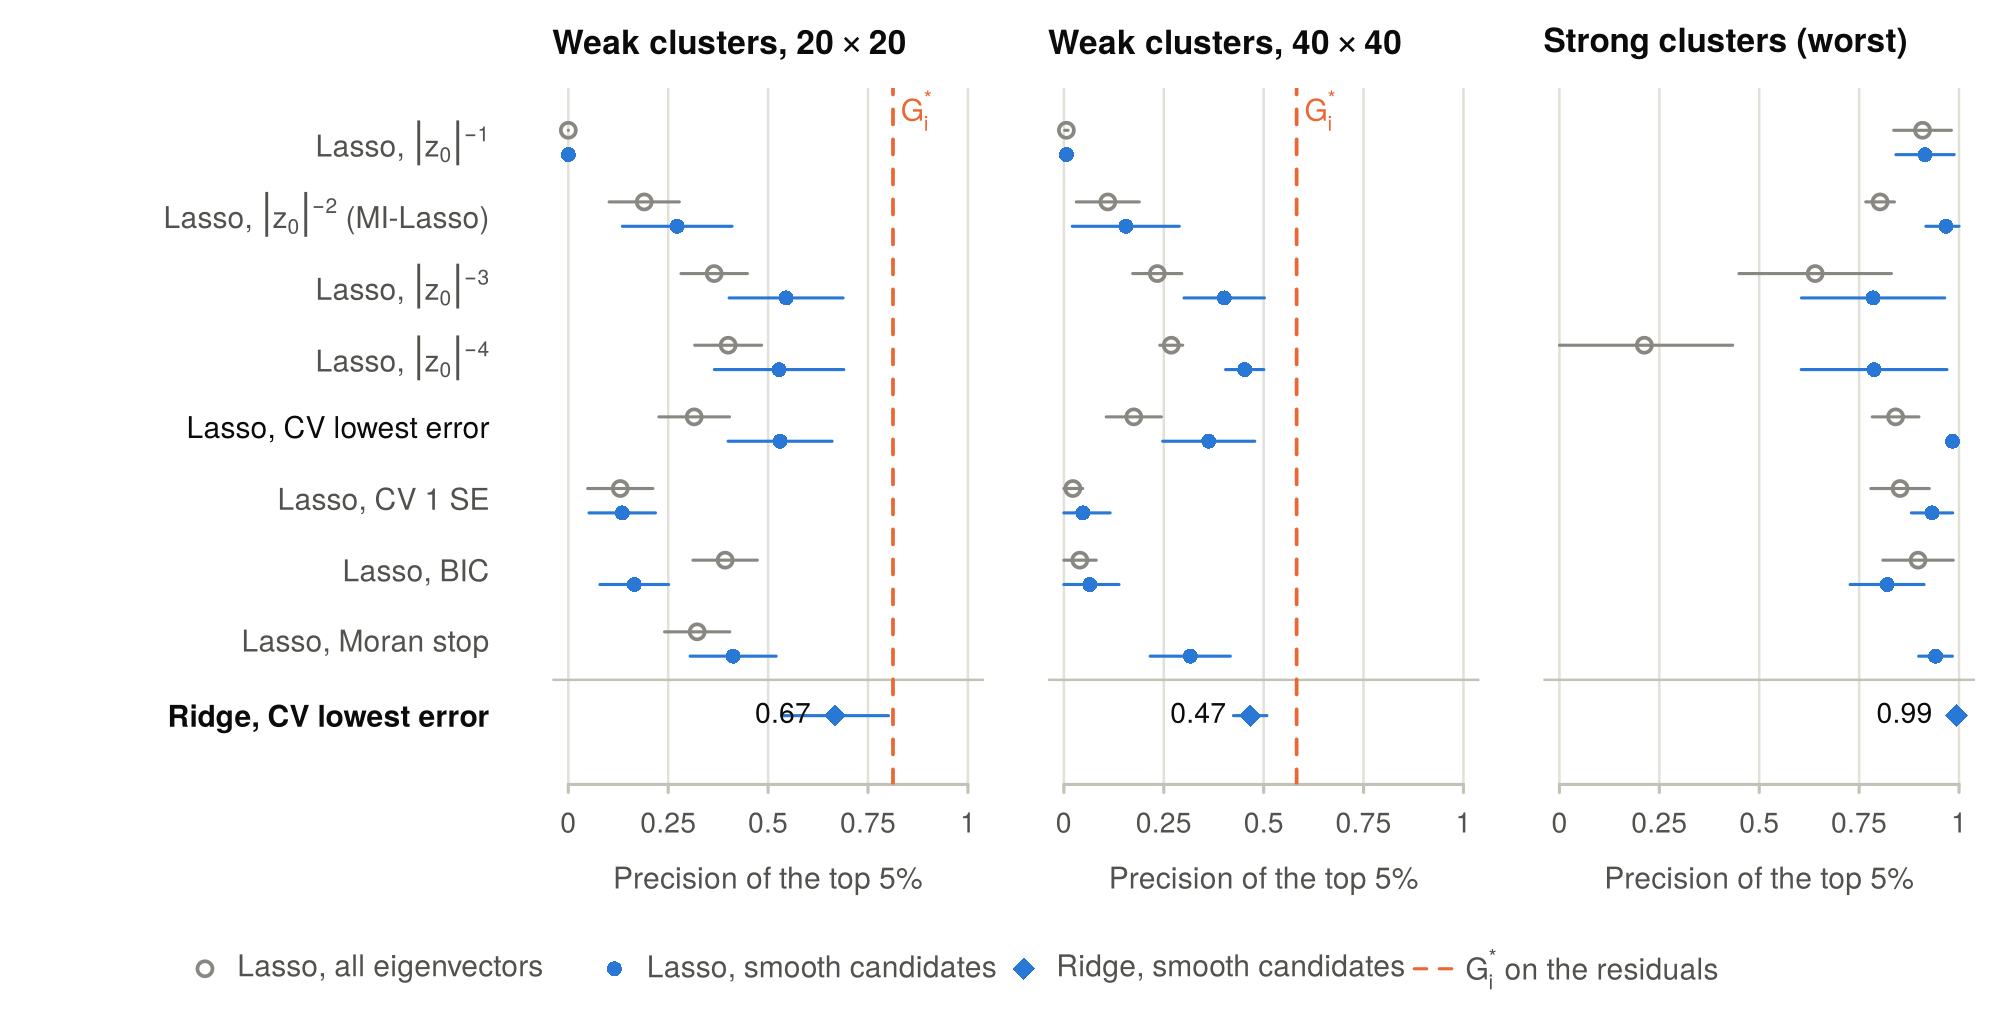
\includegraphics[width=\textwidth]{fig17_penalty_choice.png}
\caption{Choice of the estimator and of the penalty in Step~2 (choice~\ref{ch:ridge}). Precision of the top 5\% of cells for eight penalty rules for the Lasso, each with all eigenvectors (open circles) or with the smooth candidates~\eqref{eq:candidates} (filled circles), and for ridge with the cross-validated penalty on the smooth candidates (diamonds). Weak clusters: scenario B with 50 points per cluster. Strong clusters: the lowest mean over scenario A and scenario B with 500 and 200 points per cluster ($20\times20$) and with 200 points ($40\times40$). Means over 20 ($20\times20$) and 10 ($40\times40$) datasets; bars show $\pm2$ Monte Carlo standard errors. Dashed line: $G_i^*$ on the residuals of the same datasets. The Moran stop rule with all eigenvectors was not run on the $40\times40$ grid.}\label{fig:penalty}
\end{figure}

\item\label{ch:band} \textbf{Permutation band} (lines~\ref{alg:l-perm}--\ref{alg:l-label}; Step~3, equations~\eqref{eq:smoother} and~\eqref{eq:labels}).
The distribution of $\hat f_i$ under no spatial structure depends on the covariates, the candidate set and the penalty, and has no simple closed form. Permuting the residuals and applying the same smoother $S$ reproduces the estimation in each replicate, so the band accounts for the smoothing that ESF itself introduces. Because ridge is linear in $y$, this costs one matrix product rather than $B$ refits (a few seconds per dataset on the $40\times40$ grid with $B=999$, most of it for the eigendecomposition and the cross-validation). A band for the maximum of $\hat f$ over the map, which would control the chance of any false hot cell, labelled almost no cells in our simulations and was not retained.

\end{enumerate}

% Not tied to a line of the algorithm: it concerns a procedure that is no longer used.
%\paragraph{Iterative reconstruction.} The iterative reconstruction of the spatial graph and the ranking by harmonic centrality are evaluated in Appendix~\ref{app:reconstruction}. They did not improve the precision of the priority list and, without hot/cold labels, about half of the top-ranked cells were cold.

\subsection{Simulation results}\label{sec:sim-results}

%\paragraph{Measures.} 
A cell belongs to a cluster if its centre lies inside the cluster or if it contains the cluster centre. For a budget of 5\% of the cells (20 or 80 cells), we report the \emph{precision} of the priority list, the share of the selected cells that belong to a cluster, and the share of clusters with at least one selected cell. For the labels we report the share of hot cells that belong to a cluster, the share of cluster cells labelled hot, the percentage of the map labelled hot when there are no clusters (C and N), the same two shares for cold cells and the cold area (K), and the share of hot cells inside the covariate area (U).

%\paragraph{Priority list.}
 Table~\ref{tab:sim-ranking} and Figure~\ref{fig:sim-ranking} show the precision of the top 5\% of cells. With strong clusters, ESF, $G_i^*$ and LISA all reach 0.99--1.00 in scenarios B, L, M and K. Differences appear with weak clusters. With weak compact clusters (B), $G_i^*$ is the most precise (0.81 and 0.59 on the two grids), followed by LISA (0.75 and 0.52) and ESF (0.70 and 0.43). With clusters of different sizes (M), all methods select cluster cells, but ESF reaches more of the clusters: on the $40\times40$ grid it includes the smallest cluster (radius 50) in its top 5\% in 96\% (strong) and 88\% (weak) of the datasets, against 68\% and 62\% for $G_i^*$; on the $20\times20$ grid it includes the radius-100 cluster in 97--100\% of the datasets, against 79--90\% for $G_i^*$. When clusters are smaller than a cell neighbourhood (S, and E on the coarser grid), ranking the residuals without smoothing is the most precise, since both ESF and $G_i^*$ average over an area larger than the clusters. Ranking by counts fails in every scenario (precision at most 0.32): the covariate area dominates the counts, which shows that covariate adjustment is the most important step for all methods.

\begin{table}[ht]
\centering
\tiny
\caption{Precision of the top 5\% of cells (share of the selected cells that belong to a cluster), mean over replicates. Bold: highest value in the row. The three $G_i^*$ versions share the same ranking.}\label{tab:sim-ranking}
\tiny
\resizebox{\textwidth}{!}{{\tiny
\begin{tabular}{llrrrrr}
\toprule
Scenario & Grid / strength & ESF & Gi$^*$ & LISA + gate & Top residuals & Top counts \\
\midrule
B & 20$\times$20 weak & 0.70 & \textbf{0.81} & 0.75 & 0.45 & 0.00 \\
 & 20$\times$20 strong & \textbf{1.00} & 0.99 & 0.99 & 0.98 & 0.06 \\
 & 40$\times$40 weak & 0.43 & \textbf{0.59} & 0.52 & 0.27 & 0.01 \\
 & 40$\times$40 strong & 0.99 & \textbf{1.00} & 0.99 & 0.79 & 0.15 \\
\addlinespace
L & 20$\times$20 weak & 0.98 & \textbf{0.99} & 0.99 & 0.85 & 0.00 \\
 & 20$\times$20 strong & 1.00 & \textbf{1.00} & \textbf{1.00} & 1.00 & 0.08 \\
 & 40$\times$40 weak & 0.86 & \textbf{0.91} & 0.86 & 0.59 & 0.02 \\
 & 40$\times$40 strong & 1.00 & \textbf{1.00} & 1.00 & 0.95 & 0.22 \\
\addlinespace
E & 20$\times$20 weak & 0.73 & 0.70 & \textbf{0.81} & 0.73 & 0.01 \\
 & 20$\times$20 strong & 0.79 & 0.76 & 0.90 & \textbf{0.96} & 0.23 \\
 & 40$\times$40 weak & 0.74 & \textbf{0.79} & 0.74 & 0.44 & 0.04 \\
 & 40$\times$40 strong & 0.97 & 0.96 & \textbf{0.97} & 0.91 & 0.32 \\
\addlinespace
M & 20$\times$20 weak & \textbf{1.00} & 1.00 & \textbf{1.00} & 0.94 & 0.00 \\
 & 20$\times$20 strong & \textbf{1.00} & \textbf{1.00} & 1.00 & 1.00 & 0.10 \\
 & 40$\times$40 weak & 0.94 & \textbf{0.98} & 0.96 & 0.66 & 0.05 \\
 & 40$\times$40 strong & \textbf{1.00} & \textbf{1.00} & 1.00 & 0.95 & 0.25 \\
\addlinespace
S & 20$\times$20 weak & 0.17 & 0.22 & 0.28 & \textbf{0.32} & 0.01 \\
 & 20$\times$20 strong & 0.44 & 0.40 & 0.55 & \textbf{0.63} & 0.05 \\
 & 40$\times$40 weak & 0.25 & \textbf{0.31} & 0.29 & 0.17 & 0.03 \\
 & 40$\times$40 strong & \textbf{0.63} & 0.62 & 0.62 & 0.44 & 0.13 \\
\addlinespace
K & 20$\times$20 weak & \textbf{1.00} & 0.99 & 0.99 & 0.99 & 0.06 \\
 & 20$\times$20 strong & \textbf{1.00} & 0.99 & 1.00 & 0.98 & 0.06 \\
 & 40$\times$40 weak & 0.99 & \textbf{0.99} & 0.99 & 0.80 & 0.14 \\
 & 40$\times$40 strong & 0.99 & \textbf{1.00} & 0.99 & 0.81 & 0.16 \\
\addlinespace
U & 20$\times$20 weak & \textbf{0.00} & \textbf{0.00} & \textbf{0.00} & \textbf{0.00} & \textbf{0.00} \\
 & 20$\times$20 strong & 0.06 & 0.01 & 0.01 & \textbf{0.06} & \textbf{0.06} \\
 & 40$\times$40 weak & 0.00 & 0.00 & 0.00 & \textbf{0.01} & \textbf{0.01} \\
 & 40$\times$40 strong & 0.08 & 0.03 & 0.06 & \textbf{0.16} & \textbf{0.16} \\
\bottomrule
\end{tabular}
}
}
\end{table}

\begin{figure}[ht]
\centering
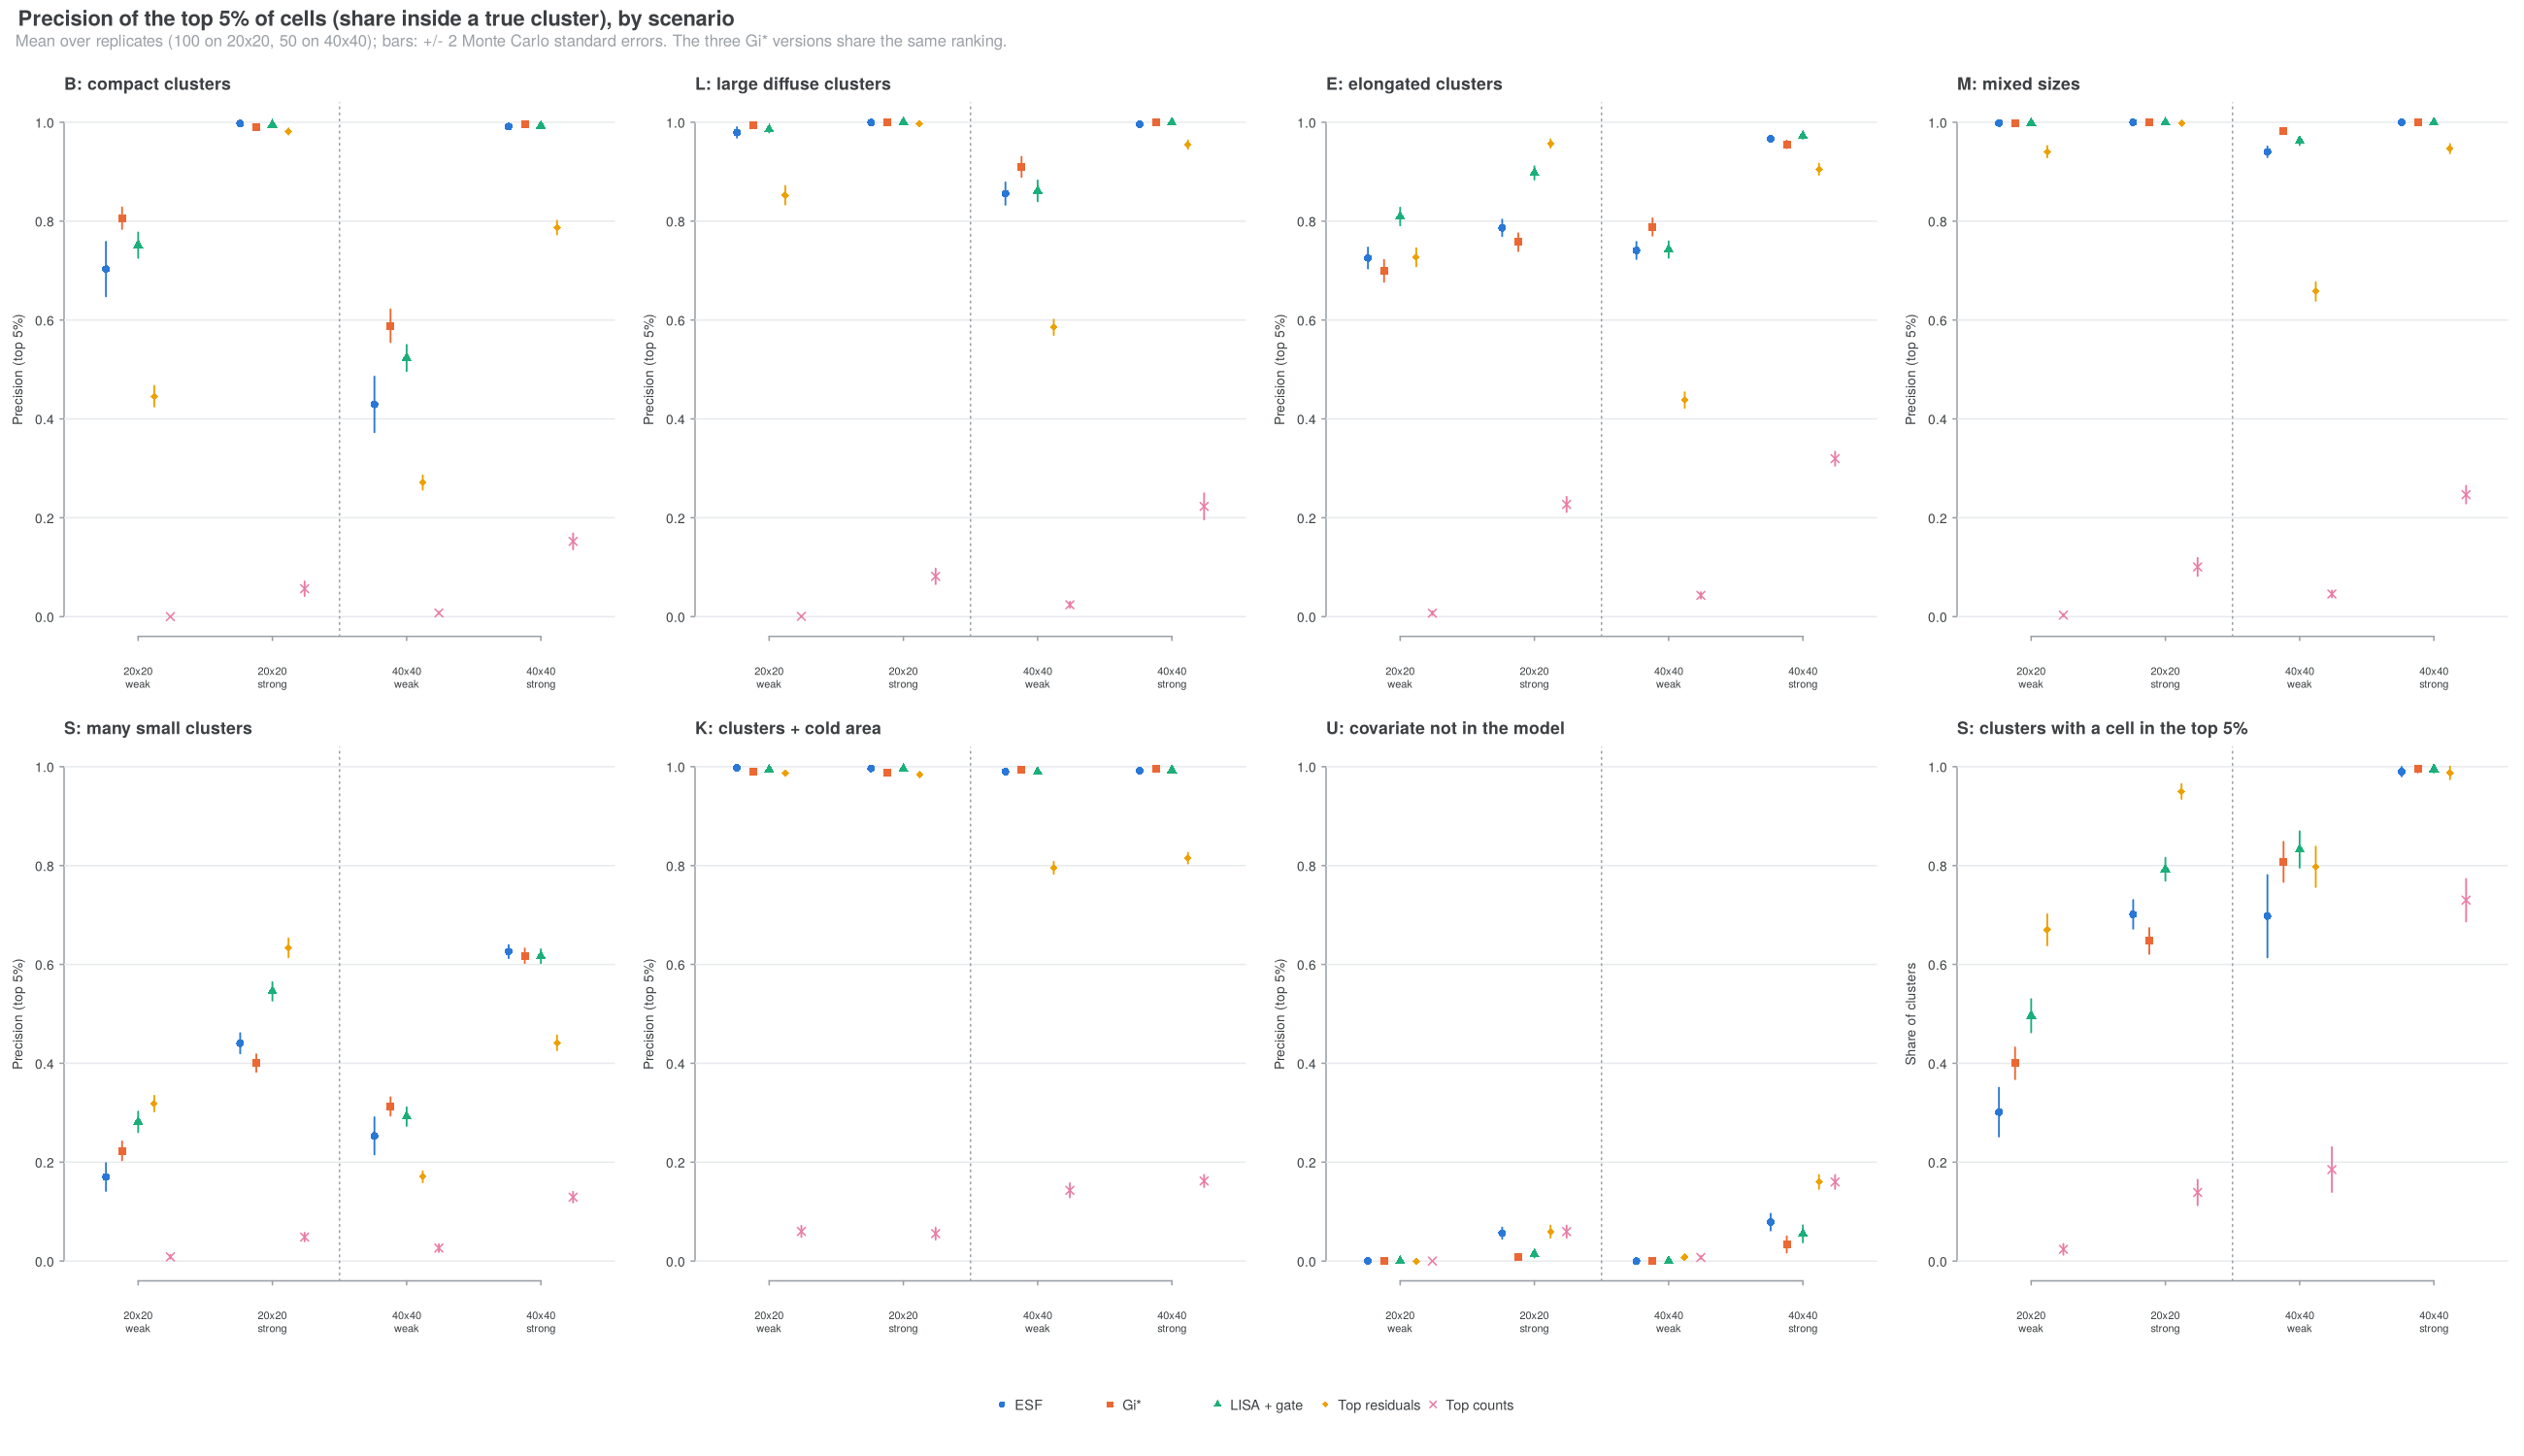
\includegraphics[width=\textwidth]{fig15_full_ranking.png}
\caption{Precision of the top 5\% of cells by scenario, grid and cluster strength; bars show $\pm2$ Monte Carlo standard errors. The last panel shows, for scenario S, the share of clusters with at least one cell in the top 5\%.}\label{fig:sim-ranking}
\end{figure}


%\paragraph{Labels.} 
Table~\ref{tab:sim-labels} and Figure~\ref{fig:sim-labels} summarise the hot and cold labels. With strong compact clusters, 78\% of the ESF hot cells belong to a cluster, against 67\% for $G_i^*$; with weak clusters the methods are within a few points of each other, and $G_i^*$ finds slightly more cluster cells. $G_i^*$ with the false discovery rate correction has the most precise labels (0.88--1.00) but finds few cluster cells when clusters are weak (1--15\%).

\begin{table}[ht]
\centering
\caption{Hot and cold labels, mean over replicates. Scenario U: lower is better.}\label{tab:sim-labels}
\small
\resizebox{\textwidth}{!}{\begin{tabular}{llrrrrr}
\toprule
Measure & Setting & ESF & Gi$^*$ & Gi$^*$ + gate & Gi$^*$ + gate + FDR & LISA + gate \\
\midrule
Hot cells inside a cluster & B strong 20$\times$20 & 0.78 & 0.67 & 0.67 & 0.88 & 0.76 \\
 & B weak 20$\times$20 & 0.60 & 0.63 & 0.62 & 0.97 & 0.68 \\
 & M strong 40$\times$40 & 0.93 & 0.91 & 0.91 & 0.99 & 0.94 \\
 & S weak 40$\times$40 & 0.28 & 0.28 & 0.29 & 1.00 & 0.31 \\
\addlinespace
Cluster cells labelled hot & B strong 20$\times$20 & 0.95 & 0.98 & 0.98 & 0.88 & 0.96 \\
 & B weak 20$\times$20 & 0.54 & 0.63 & 0.58 & 0.15 & 0.46 \\
 & M strong 40$\times$40 & 0.87 & 0.92 & 0.92 & 0.79 & 0.84 \\
 & S weak 40$\times$40 & 0.35 & 0.44 & 0.35 & 0.01 & 0.28 \\
\addlinespace
\% of cells hot, no clusters & C 20$\times$20 & 1.4 & 5.6 & 1.2 & 0.0 & 0.8 \\
 & N 20$\times$20 & 0.2 & 4.0 & 0.2 & 0.0 & 0.1 \\
 & C 40$\times$40 & 2.0 & 5.3 & 1.9 & 0.0 & 1.3 \\
 & N 40$\times$40 & 1.0 & 4.6 & 0.8 & 0.0 & 0.5 \\
\addlinespace
Cold cells inside the cold area & K strong 20$\times$20 & 0.81 & 0.70 & 0.70 & 0.88 & 0.81 \\
 & K strong 40$\times$40 & 0.62 & 0.58 & 0.58 & 0.93 & 0.74 \\
\addlinespace
Cold-area cells labelled cold & K strong 20$\times$20 & 0.97 & 1.00 & 1.00 & 0.96 & 0.98 \\
 & K strong 40$\times$40 & 0.87 & 0.96 & 0.96 & 0.80 & 0.85 \\
\addlinespace
Hot cells in the covariate area & U strong 20$\times$20 & 0.56 & 0.48 & 0.48 & 0.63 & 0.53 \\
 & U strong 40$\times$40 & 0.56 & 0.51 & 0.51 & 0.64 & 0.55 \\
\bottomrule
\end{tabular}
}
\end{table}



\begin{figure}[ht]
\centering
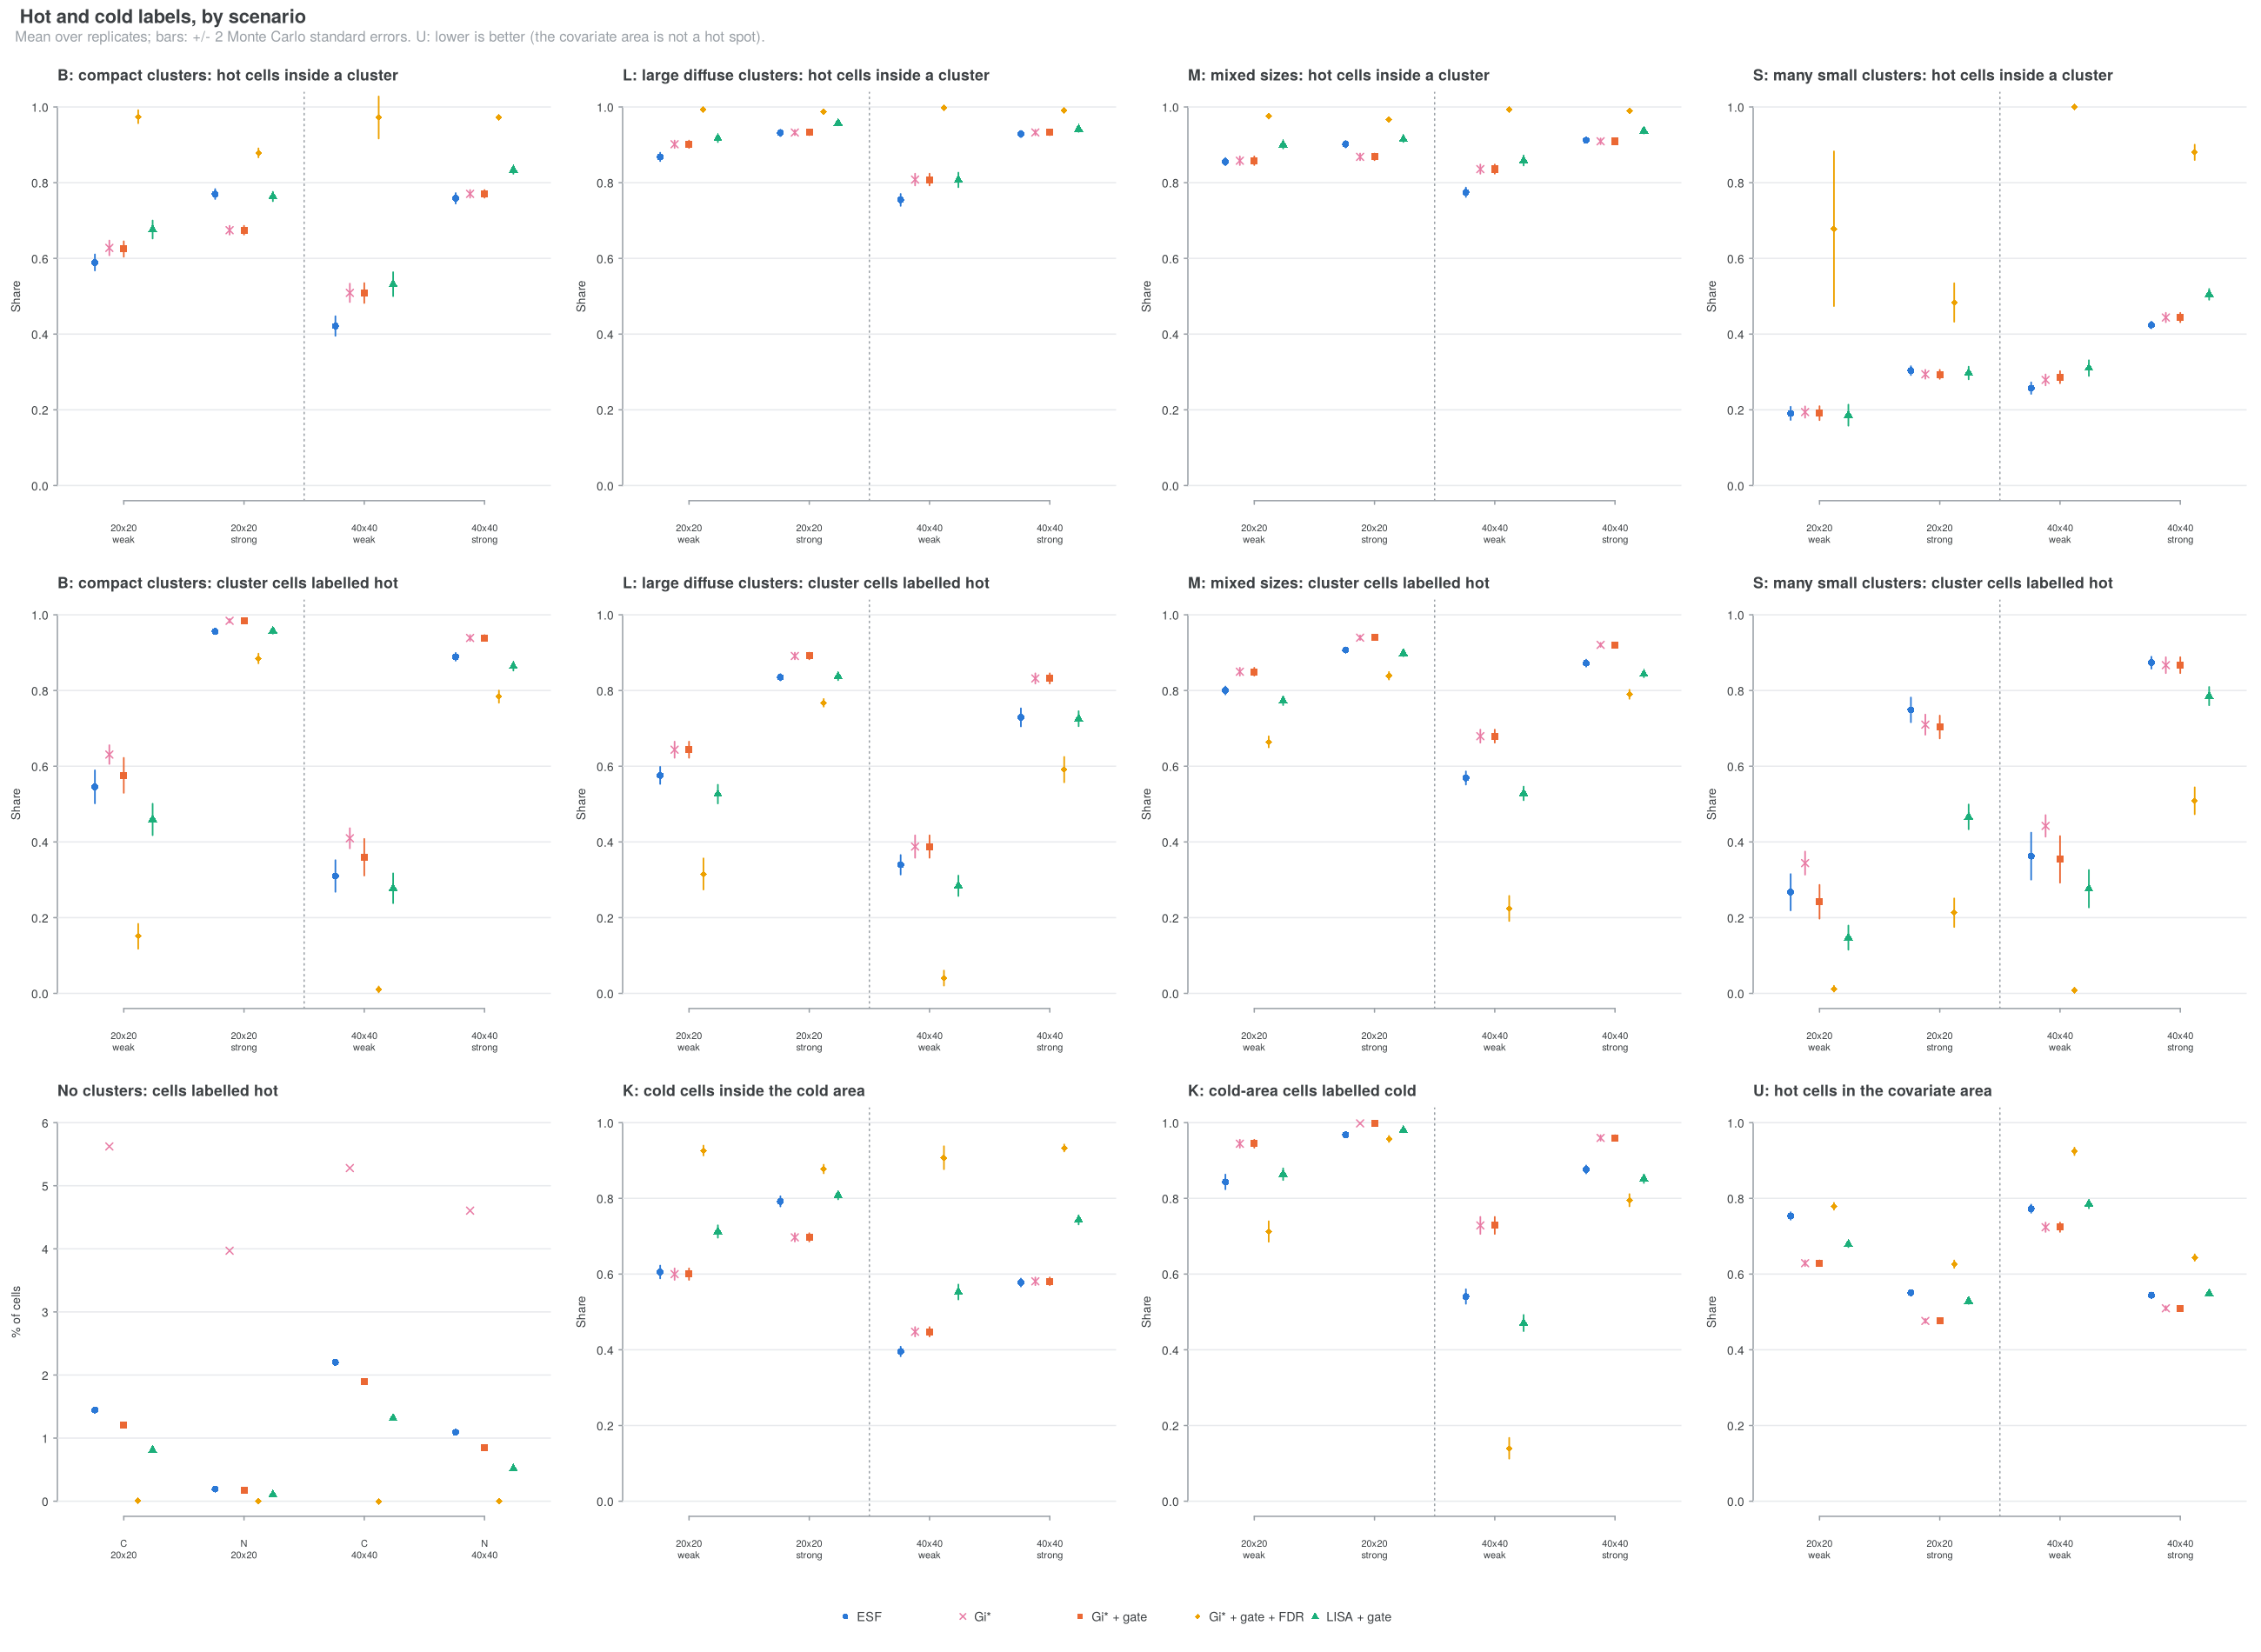
\includegraphics[width=\textwidth]{fig16_full_labels.png}
\caption{Hot and cold labels by scenario: share of hot cells inside a cluster, share of cluster cells labelled hot, percentage of the map labelled hot without clusters (C, N), cold labels in scenario K, and hot cells in the covariate area when the covariate is missing (U).}\label{fig:sim-labels}
\end{figure}


%\paragraph{No clusters.} 
Without the test of Step~1, $G_i^*$ labels 4.0--5.6\% of the map hot in scenarios C and N, as expected from its 5\% level. With the test, ESF labels 0.2--2.0\% hot, $G_i^*$ 0.2--1.9\% and LISA 0.1--1.3\%. The test therefore provides most of the protection against false hot spots, for all local methods. It rejects in 3\% of the datasets with random points on the $20\times20$ grid, and in 19\% (C, $20\times20$) and 32\% (C, $40\times40$) of the datasets that contain only the covariate area. The rejections in C occur because the covariate enters the model linearly while its effect on $\log(1+w)$ is not linear; a spline for each covariate reduced them to 4--6\%, at the cost of power with weak clusters (Section~\ref{sec:sim-choices}). On random points with the $40\times40$ grid the test rejected in 8 of 50 datasets; a check with 500 further datasets gave 5.0\% (95\% interval 3.3--7.3\%), so the test holds its level.

%\paragraph{Cold areas.} 
In scenario K with a strong cold area, ESF labels 97\% ($20\times20$) and 87\% ($40\times40$) of the cold-area cells cold, and 81\% and 62\% of its cold cells lie in the cold area. $G_i^*$ labels more of the cold area (100\% and 96\%), but a lower share of its cold cells lies inside it (70\% and 58\%); LISA has the most precise cold labels among the methods without the correction (81\% and 74\%). Outside the cold area, cold labels mark cells with few points by chance, which is more frequent on the finer grid.

%\paragraph{Missing covariate.}
 When the model does not receive the covariate (U), every method fails in the same way: about half of the hot cells (48--64\%) and most of the top 5\% (82--99\%) fall in the covariate area. A hot spot is only defined relative to the covariates that are in the model, which is why the choice of covariates in the application deserves care.




\section{Application to cockroach sightings in Madrid}\label{sec:app}
\todo{data and grid; exposure and covariates (Tamayo-Uria et al.; Ayyad et al.); nested models M1--M3 and rats; maps per summer and persistence; out-of-sample table (\texttt{madrid\_final\_out\_of\_sample.tex}); grid size.}

\section{Discussion}\label{sec:conc}
\todo{main findings; when to use ESF or local statistics; limitations: reports are not abundance, covariates and sightings from different years, field-campaign variables, non-linear covariate effects and the test, grid size \citep{openshaw1984modifiable}; extensions (space--time).}


\section*{Declarations}
\subsection*{Funding}
YC and CA gratefully acknowledge the support provided by the Escuela Politécnica Nacional of Ecuador, for the development of the project PII-DM-2024-02 \textit{``Modelamiento de interacción espacial de dos especies o grupos mediante método MiLasso''}. J. Mateu is partially funded by projects CIAICO/2022/191 from Generalitat Valenciana and PID2022-141555OB-I00 from Ministry of Science and Innovation.
\subsection*{Declaration of conflicting interests}
All authors declared no potential conflicts of interest with respect to the research, authorship and/or publication of this article.
\subsection*{Author contributions}
\todo{update}
\subsection*{Use of artificial intelligence}
During the revision, the authors used Claude (Anthropic), a large language model used through an agentic coding and writing environment, as a research assistant. Under the authors' direction, Claude: reorganised the analysis code into an R package and wrote unit tests; implemented the proposed procedure and the benchmark methods ($G_i^*$, local Moran's $I$ and the rankings without smoothing); proposed and ran, after discussion with the authors, the simulation experiments of Section~\ref{sec:sim}; prepared the Madrid data (grid, exposure and covariates), ran the analyses of Section~\ref{sec:app}, and checked the covariate definitions against the cited sources; produced the figures and tables; and drafted the text of the Methods and Simulation sections and of Appendix~\ref{app:reconstruction}. All modelling decisions (choice of method, penalty, test, scenarios, data and covariates) were taken by the authors. The authors checked the code, verified the reported numbers against the outputs, and reviewed and edited all text. The authors take full responsibility for the content of this article. Claude is not an author.

\bibliographystyle{CUP}
\bibliography{referencias,referencias_new}

\newpage
\begin{appendices}
% =====================================================================
% Appendix: iterative reconstruction of the spatial weights matrix
%
% Usage in the main paper (after \appendix):
%     % =====================================================================
% Appendix: iterative reconstruction of the spatial weights matrix
%
% Usage in the main paper (after \appendix):
%     % =====================================================================
% Appendix: iterative reconstruction of the spatial weights matrix
%
% Usage in the main paper (after \appendix):
%     \input{appendix_reconstruction}
% Figures are read from ../simulation/figures/ (set in the preamble with
%     \graphicspath{{../simulation/figures/}}
% or copy the PNG files next to the .tex file).
% Packages used: graphicx, amsmath (both loaded by sn-jnl).
% Figures and tables are produced by simulation/04_iteration_figures.R from the
% results of simulation/01_ ... 06_*.R in the project repository.
% =====================================================================

\section{Iterative reconstruction of the spatial weights matrix}
\label{app:reconstruction}

This appendix describes an extension of the eigenvector spatial filtering (ESF) step that reconstructs a sparser spatial weights matrix from the selected eigenvectors and iterates the selection on the reconstructed graph. We evaluate it in simulation and explain why it is not part of the proposed procedure.

\subsection{The iterative reconstruction}
\label{app:rec-procedure}

Let $A$ be the $n\times n$ binary contiguity matrix of the study region, $Y$ the standardised counts per cell and $Z$ the standardised covariates. The procedure starts from $D^{(0)}=A$ and, at iteration $k$:

\begin{enumerate}
  \item computes the eigendecomposition $D^{(k)} = E\,\Delta\,E^\top$, with $\Delta=\mathrm{diag}(\delta_1,\dots,\delta_n)$, and selects a subset $S$ of eigenvectors with the MI-Lasso estimator, with penalty $\lambda=|z_0|^{-2}$ fixed from the standardised Moran's $I$ of the residuals of $Y$ on $Z$;
  \item reconstructs
  \begin{equation}
    B = E_S\,\Delta_S\,E_S^\top, \qquad b_{ij} = \sum_{s\in S}\delta_s\, e_s(i)\, e_s(j);
    \label{eq:app-B}
  \end{equation}
  \item applies a rounding rule: among the edges of $D^{(k)}$ with $b_{ij}>0$, it keeps those with $b_{ij}\ge\tau^{(k)}$, where $\tau^{(k)}$ is a threshold computed from these values, giving $D^{(k+1)} = D^{(k)}\circ\mathbf{1}\{B\ge\tau^{(k)}\}$;
  \item accepts $D^{(k+1)}$ if the post-Lasso residuals obtained with its eigenvectors show no spatial correlation (Moran's $I$ with $A$, level $0.05$), and stops otherwise or when $D^{(k+1)}=D^{(k)}$.
\end{enumerate}

Because each accepted step removes at least one edge, the procedure stops after at most as many iterations as $A$ has edges. Cells are then ranked by a ranking rule applied to the final graph.

We call \emph{baseline configuration} the procedure with all $n$ eigenvectors as candidates, eigenvalue weights in \eqref{eq:app-B}, the 75\% quantile of the positive $b_{ij}$ as threshold, and cells ranked by harmonic centrality on the final graph. Each variant below changes one element of the baseline.

\paragraph{Rounding rules.}
\emph{None} (all edges kept, $D=A$; no reconstruction);
\emph{quantile $q$} ($\tau$ = $q$-quantile of the positive $b_{ij}$ on the current edges, $q\in\{0.50, 0.75, 0.80, 0.90\}$);
\emph{mixture} (a two-component Gaussian mixture fitted to the positive $b_{ij}$; $\tau$ is the point between the two means where the weighted component densities are equal, and all edges are kept when the Bayesian information criterion selects one component);
\emph{permutation} (30 Freedman--Lane permutations of the residuals of $Y$ on $Z$; for each, the selection and \eqref{eq:app-B} are recomputed on the current graph, and $\tau$ is the 95th percentile of the pooled positive $b_{ij}$).

\paragraph{Ranking rules.}
Let $\hat f = E_S\hat\gamma_S$ be the fitted spatial component (centred), and call a cell \emph{hot} if $\hat f_i>0$ and \emph{cold} otherwise.
\emph{Centrality, whole graph}: harmonic centrality on the final graph, over all cells (baseline).
\emph{Centrality, hot cells}: harmonic centrality computed among hot cells only.
\emph{Largest excess}: hot cells ordered by $\hat f_i$.
\emph{Hot zones first}: connected groups of hot cells ordered by $\sum_{i}\hat f_i$; within a group, cells ordered by harmonic centrality.
Two benchmarks that do not use the graph are also reported: \emph{top counts} (cells ordered by $Y$) and \emph{top residuals} (cells ordered by the residuals of $Y$, or of $\log(Y+1)$, on $Z$).

\subsection{Simulation design}
\label{app:rec-design}

All scenarios use a $1000\times1000$ window divided into a regular grid with queen contiguity. Table~\ref{tab:app-scenarios} lists the scenarios.

\begin{table}[ht]
\centering
\caption{Simulated scenarios.}
\label{tab:app-scenarios}
\begin{tabular}{p{0.16\textwidth}p{0.50\textwidth}p{0.24\textwidth}}
\hline
Scenario & Data-generating process & Target \\
\hline
A: clusters & Three clusters: parents uniform in the window at least 100 units from the border; 500 offspring per parent, uniform in a disc of radius 100; 2000 additional uniform points. No covariate. & Cells inside the three discs \\
B: clusters and covariate & Scenario A plus 3000 points accepted with probability $\exp\{3(b(x)-1)\}$, where $b$ is a Gaussian surface (standard deviation 150) centred at least 300 units from every parent. The model receives $Z=(b,\ \varepsilon)$ at the cell centres, with $\varepsilon\sim N(0,1)$. & Cells inside the three discs, not the covariate area \\
D: barriers & $Y=\rho W Y + Z\beta + e$ on a $20\times20$ grid, with $W$ the row-standardised version of a graph $W^\ast\subset A$ in which a vertical line (one crossing left open) and a horizontal line on the left half remove 85 of the 1482 edges; $Z$ a linear gradient and noise, $\beta=(1,0)$, $\rho\in\{0.5,0.8,0.95\}$. & The 85 removed edges \\
D0: no barriers & As D with $W^\ast=A$. & No edge removed \\
\hline
\end{tabular}
\end{table}

Unless stated otherwise the grid has $20\times20$ cells (cell side 50) and the budget is the top 20 cells (5\%). For scenarios A and B, \emph{precision} is the share of the selected cells inside a true cluster disc. For scenarios D and D0, edges are classified as kept or removed, and we report the area under the ROC curve (AUC) of $b_{ij}$ for separating real from barrier edges, the share of edges kept, and Youden's $J$ = (share of barrier edges removed) + (share of real edges kept) $-\,1$, which is 0 for a classification unrelated to the barriers.

\subsection{Results}
\label{app:rec-results}

\paragraph{Sign of the reconstructed weights.}
Equation~\eqref{eq:app-B} is invariant to the sign of each eigenvector, since $e_s e_s^\top=(-e_s)(-e_s)^\top$. A positive $b_{ij}$ indicates that cells $i$ and $j$ lie on the same side of the selected spatial patterns, whether both have high or both have low counts. Under the baseline configuration, half of the 20 cells ranked highest in scenario B had $\hat f_i<0$, and precision was 0.28 in scenario A and 0.24 in scenario B (Fig.~\ref{fig:app-cold}). Ranking hot cells by $\hat f$ gave 1.00 and 0.96. Figure~\ref{fig:app-example} shows the successive graphs and the selected cells for one simulated map.

\begin{figure}[ht]
\centering
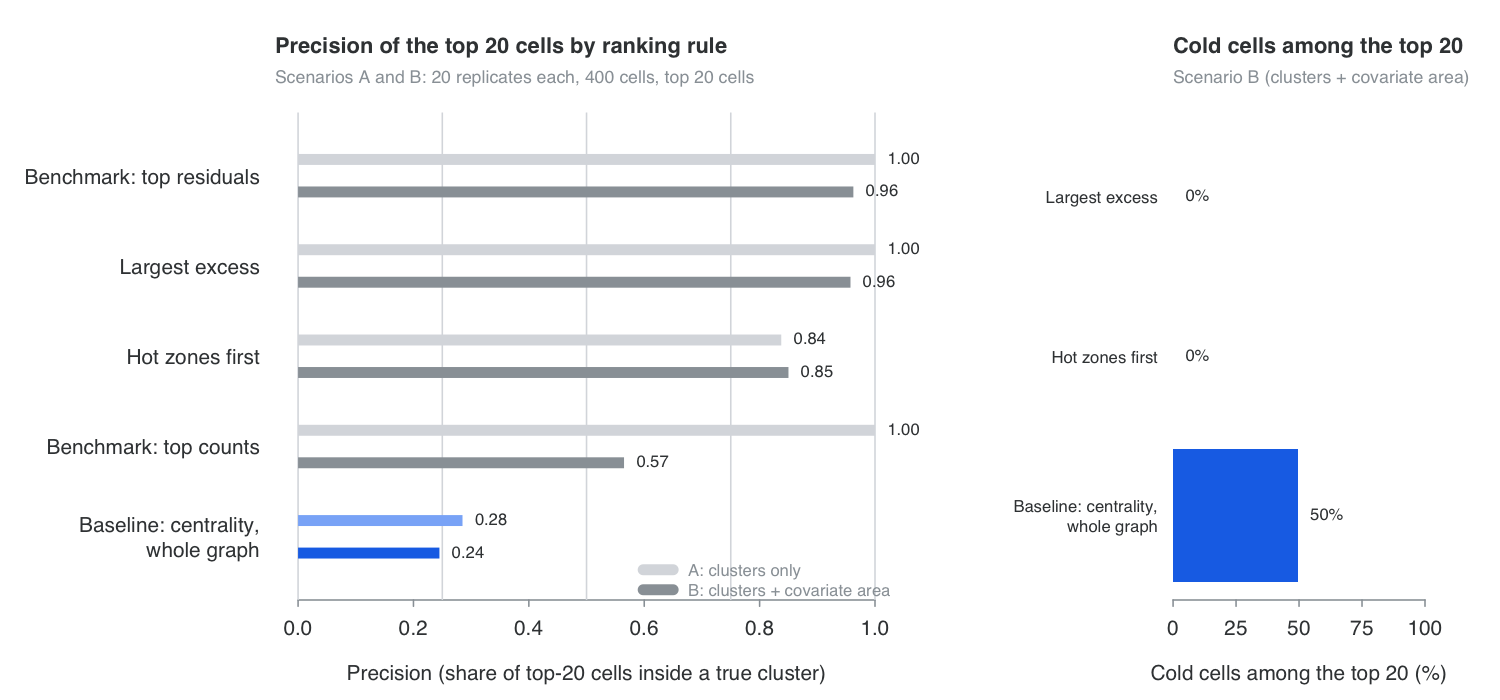
\includegraphics[width=\textwidth]{fig1_cold_zones}
\caption{Precision of the top 20 of 400 cells by ranking rule (scenarios A and B, 20 replicates each) and share of cold cells among them (scenario B). Baseline: harmonic centrality on the final graph.}
\label{fig:app-cold}
\end{figure}

\begin{figure}[ht]
\centering
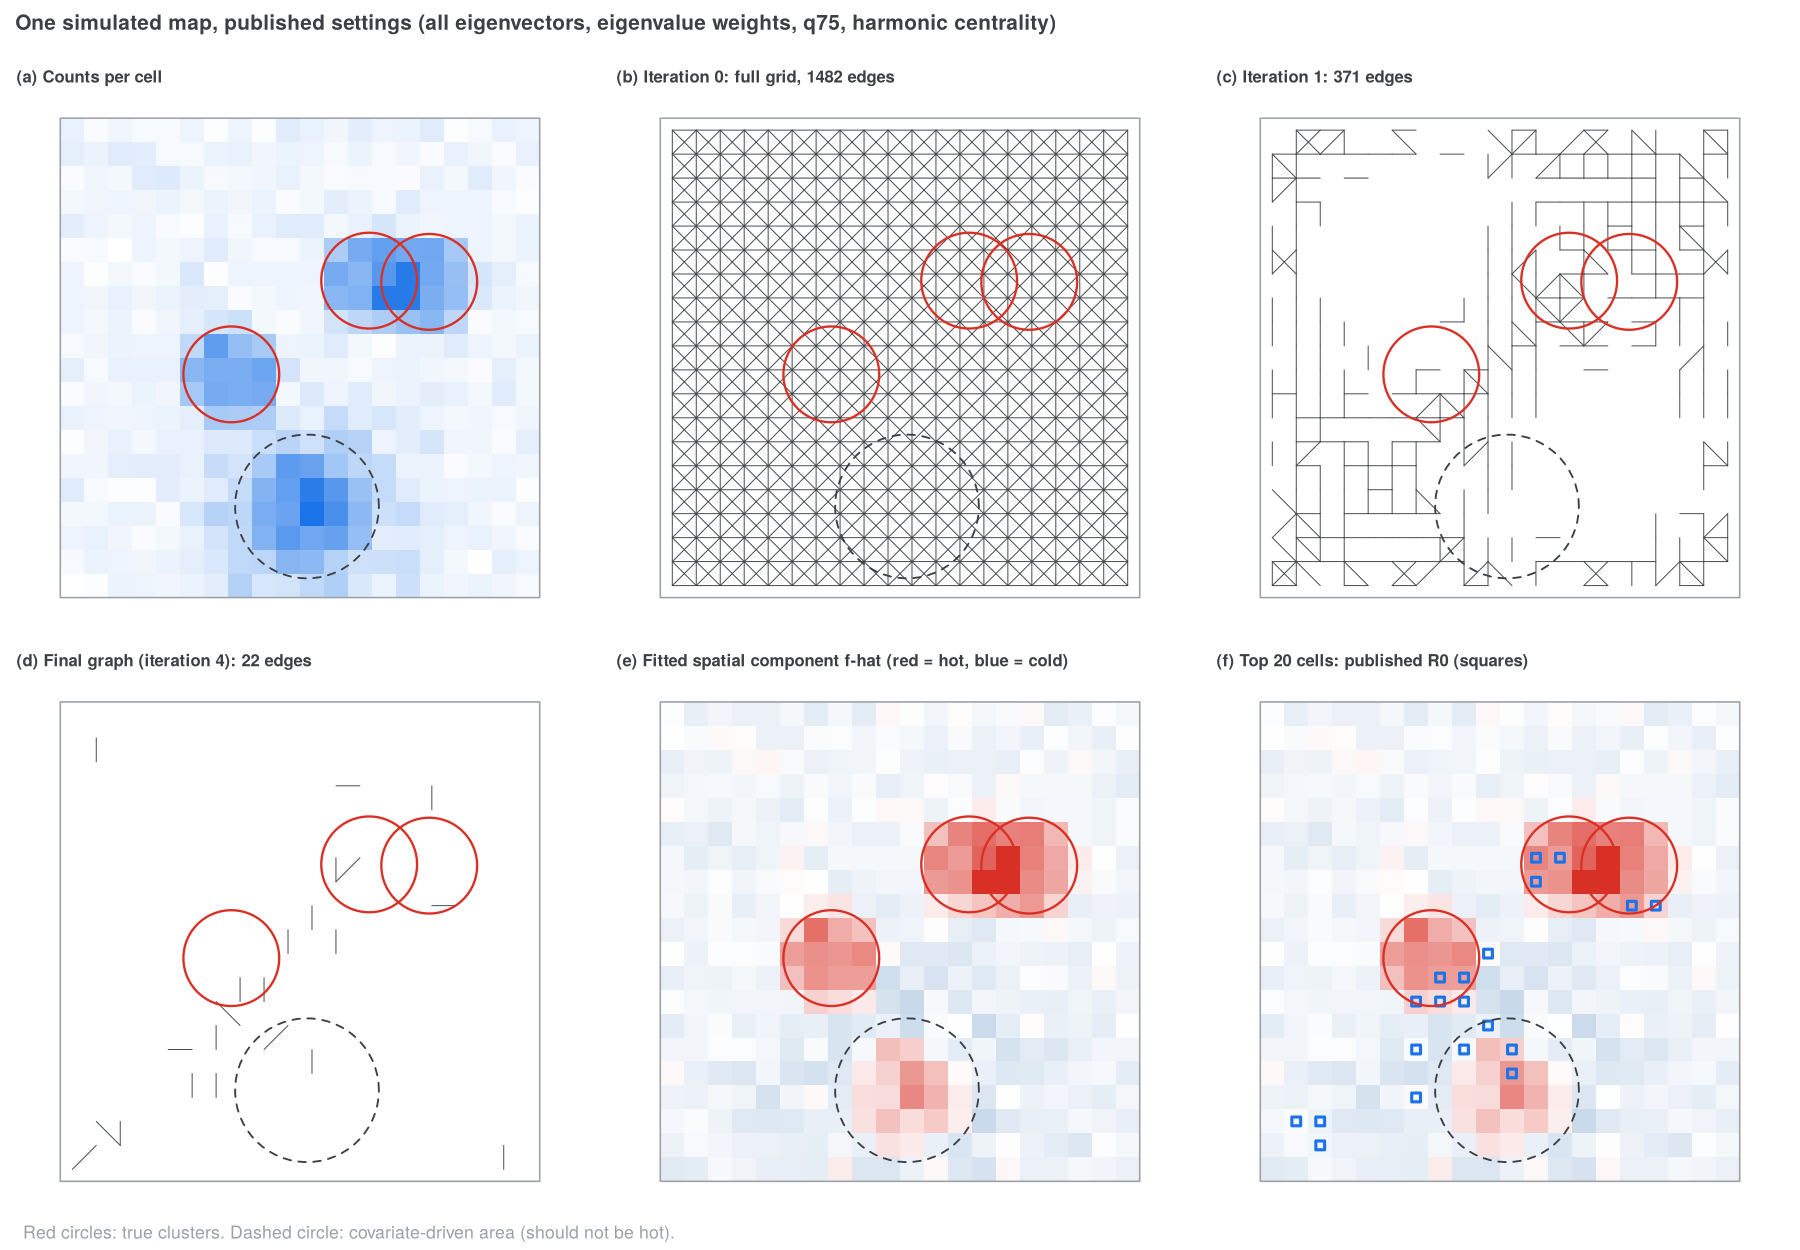
\includegraphics[width=\textwidth]{figS2_example_run}
\caption{One simulated map from scenario B under the baseline configuration. (a) Counts per cell. (b)--(d) Graph at iterations 0, 1 and at the last accepted iteration. (e) Fitted spatial component $\hat f$. (f) Top 20 cells under the baseline ranking. Circles: true clusters; dashed circle: covariate area.}
\label{fig:app-example}
\end{figure}

\paragraph{Effect of rounding and iteration on the selected cells.}
We compared rounding with the 75\% quantile against no rounding over 162 settings of scenario B: grids of $10\times10$, $20\times20$ and $40\times40$ cells, 50, 200 or 500 points per cluster, penalty exponents $a\in\{0.5,1,2\}$ in $\lambda=|z_0|^{-a}$, counts on the original or the $\log(Y+1)$ scale, and three ranking rules (10 replicates per setting). Iteration removed edges in 495 of 1620 runs (31\%); in the remaining runs the first reduced graph was rejected by the Moran test. In the runs where edges were removed, the change in precision was $+0.06$ (95\% CI $0.02$ to $0.10$) for centrality on the whole graph, $-0.01$ ($-0.03$ to $0.01$) for largest excess and $-0.06$ ($-0.11$ to $-0.01$) for hot zones first (Fig.~\ref{fig:app-iteration}).

\begin{figure}[ht]
\centering
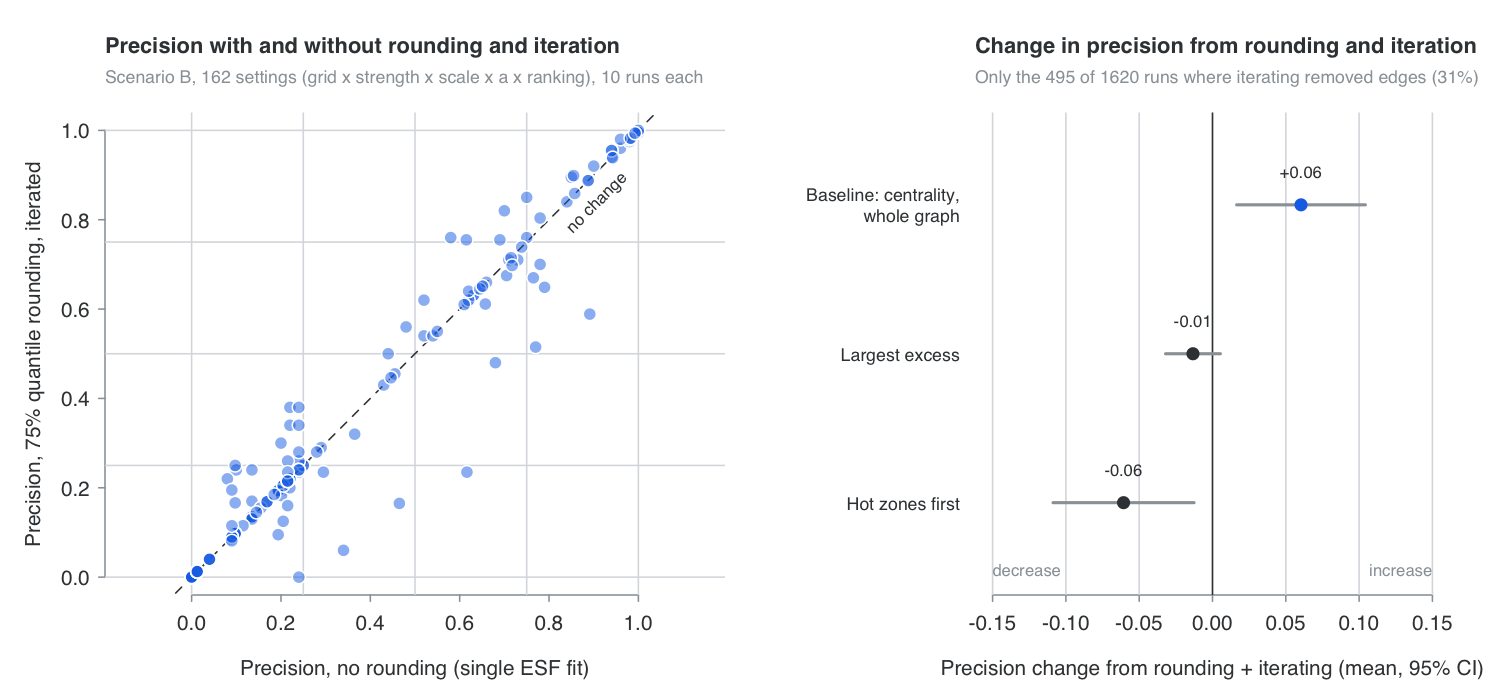
\includegraphics[width=\textwidth]{fig2_iteration_no_effect}
\caption{Left: precision with no rounding against precision with 75\% quantile rounding and iteration; each point is one setting (mean of 10 replicates). Right: change in precision in the runs where iteration removed edges (mean and 95\% confidence interval).}
\label{fig:app-iteration}
\end{figure}

\paragraph{Rounding rules.}
Table~\ref{tab:app-rounding} and Fig.~\ref{fig:app-rounding} compare the seven rounding rules with all other elements fixed at the baseline (scenarios A and B, 20 replicates each; scenarios D and D0, 20 replicates each). With the largest-excess ranking, precision was 1.00 in scenario A and 0.95--0.96 in scenario B for every rule, including no rounding. With hot zones first, the 80\% and 90\% quantiles and the permutation rule gave about 0.10 more than no rounding, and remained below the largest-excess ranking. With the baseline ranking, precision ranged from 0.10 to 0.37. In scenario D0 every rule except the mixture removed between 90\% and 97\% of the edges.

\begin{table}[ht]
\centering
\caption{Precision of the top 20 cells (scenario A / scenario B) by rounding rule and ranking rule, and share of edges kept in scenario D0. Mean of 20 replicates.}
\label{tab:app-rounding}
\small\setlength{\tabcolsep}{4pt}
\begin{tabular}{lcccc}
\hline
Rounding rule & Largest excess & Hot zones first & Centrality, & Edges kept \\
 & & & whole graph & (D0) \\
\hline
None            & 1.00 / 0.95 & 0.85 / 0.76 & 0.13 / 0.10 & 100\% \\
50\% quantile   & 1.00 / 0.95 & 0.81 / 0.71 & 0.32 / 0.37 & 6\% \\
75\% quantile (baseline) & 1.00 / 0.95 & 0.84 / 0.84 & 0.22 / 0.29 & 8\% \\
80\% quantile   & 1.00 / 0.95 & 0.89 / 0.90 & 0.19 / 0.31 & 3\% \\
90\% quantile   & 1.00 / 0.95 & 0.91 / 0.91 & 0.26 / 0.32 & 10\% \\
Mixture         & 1.00 / 0.96 & 0.80 / 0.78 & 0.26 / 0.31 & 76\% \\
Permutation     & 1.00 / 0.95 & 0.90 / 0.91 & 0.23 / 0.37 & 10\% \\
\hline
\end{tabular}
\end{table}

\begin{figure}[ht]
\centering
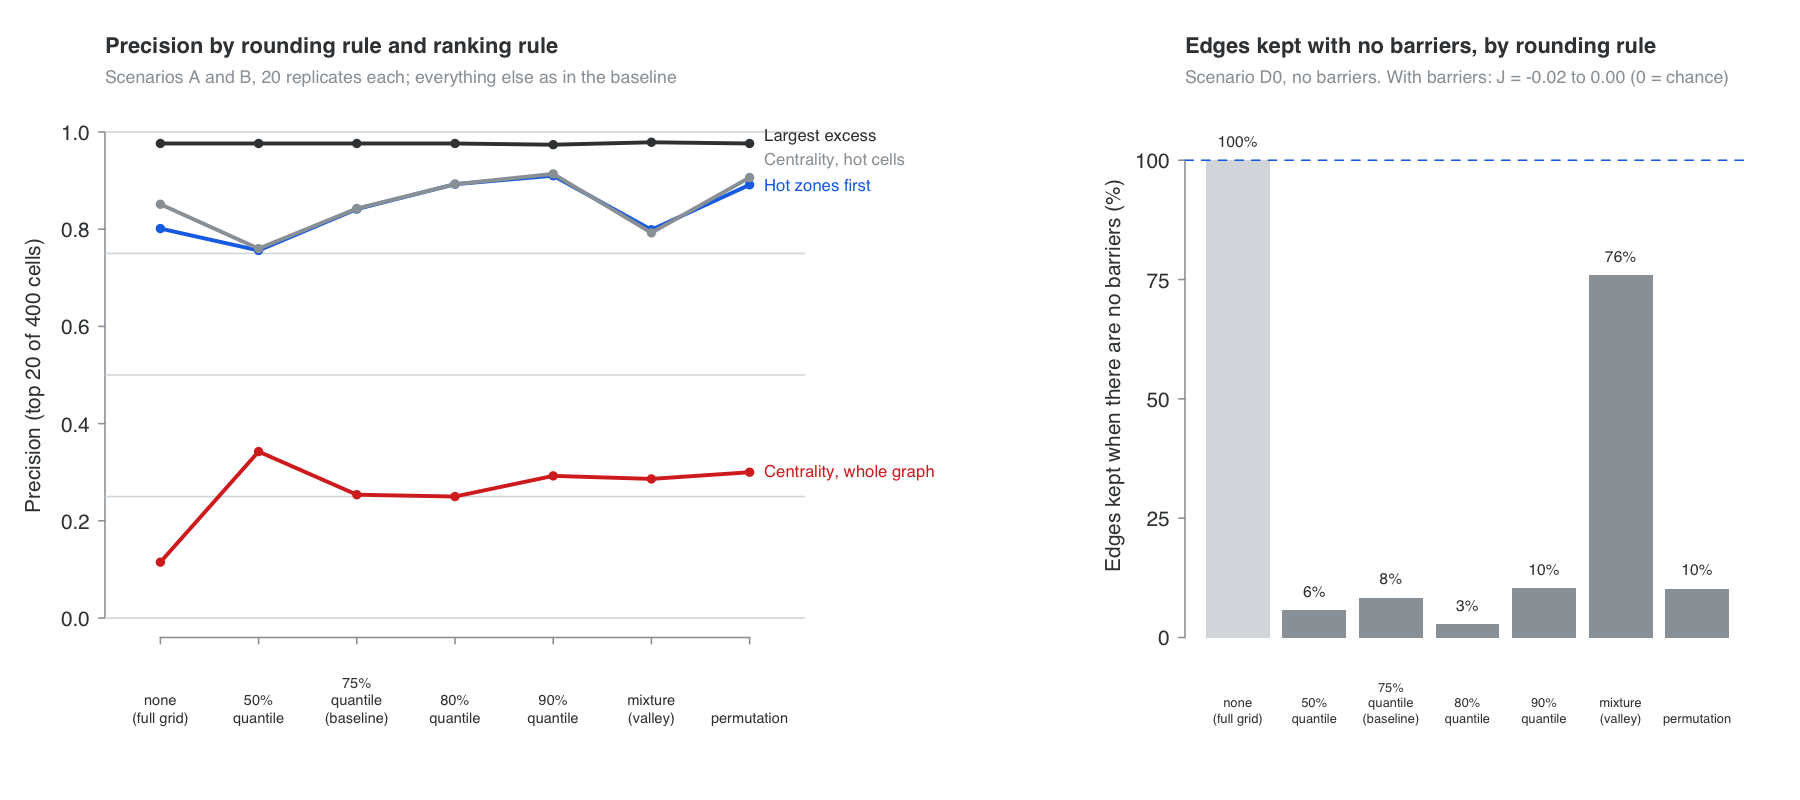
\includegraphics[width=\textwidth]{fig4_rounding_rules}
\caption{Left: precision of the top 20 of 400 cells by rounding rule and ranking rule (scenarios A and B pooled, 20 replicates each). Right: share of edges kept in scenario D0, where no edge should be removed. Rules: none (full grid), q50--q90 (quantile of the positive $b_{ij}$; q75 is the baseline), mix (two-component mixture), perm (permutation).}
\label{fig:app-rounding}
\end{figure}

\paragraph{Fine grid with weak clusters.}
On a $40\times40$ grid (cell side 25) with 50 or 200 points per cluster, scenario B, budget of 80 cells, 10 replicates, the rankings that use hot cells and connectivity reached, with no rounding, a precision of 0.44--0.48 (50 points) and 0.81--0.89 (200 points), against 0.29 and 0.80 for top residuals on the log scale. Rounding reduced the precision of hot zones first by 0.24 and 0.25 (75\% quantile), 0.18 and 0.17 (90\% quantile) and 0.06 and 0.10 (permutation) (Fig.~\ref{fig:app-finegrid}).

\begin{figure}[ht]
\centering
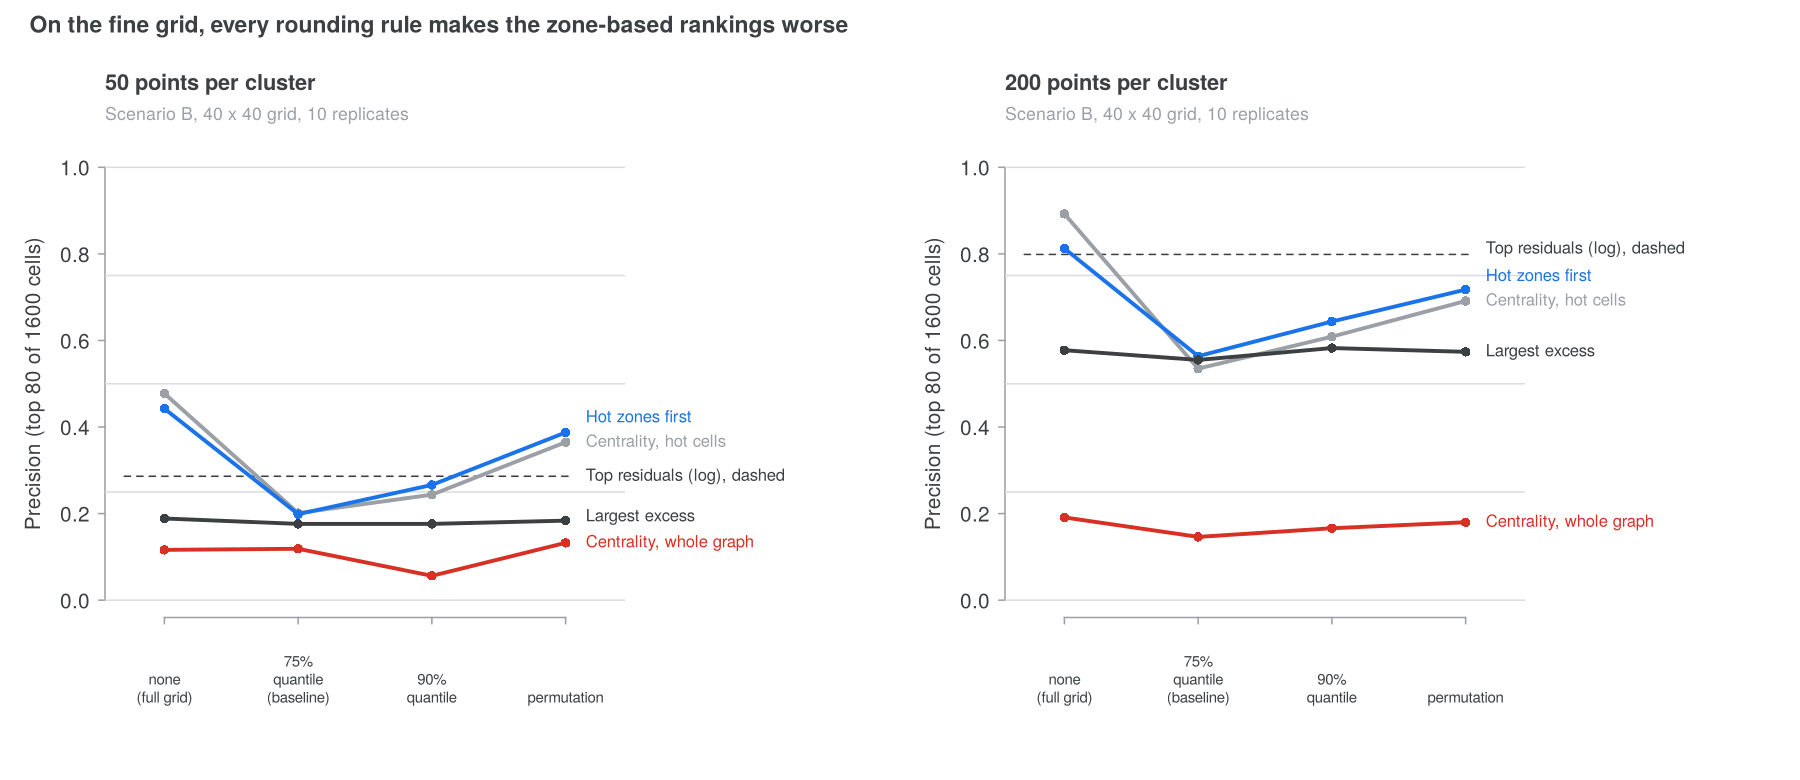
\includegraphics[width=\textwidth]{fig5_fine_grid}
\caption{Precision of the top 80 of 1600 cells by rounding rule and ranking rule on a $40\times40$ grid (scenario B, 10 replicates per panel). Dashed line: top residuals of $\log(Y+1)$ on $Z$. Rule labels as in Figure~\ref{fig:app-rounding}.}
\label{fig:app-finegrid}
\end{figure}

\paragraph{Recovery of a known graph.}
In scenario D, the AUC of $b_{ij}$ for separating real from barrier edges was 0.55, 0.55 and 0.45 for $\rho=0.5$, $0.8$ and $0.95$ with eigenvalue weights, and 0.55, 0.53 and 0.61 with squared coefficients $\hat\gamma_s^2$ as weights. The absolute difference between the residuals of neighbouring cells, $|e_i-e_j|$, gave 0.55, 0.65 and 0.96 (Fig.~\ref{fig:app-graph}). After the full procedure, Youden's $J$ ranged from $-0.02$ to $0.00$ across rounding rules. With 130--300 of 400 eigenvectors selected, $B$ differs from $A$ by a small number of patterns with global support, while a barrier is a local discontinuity.

\begin{figure}[ht]
\centering
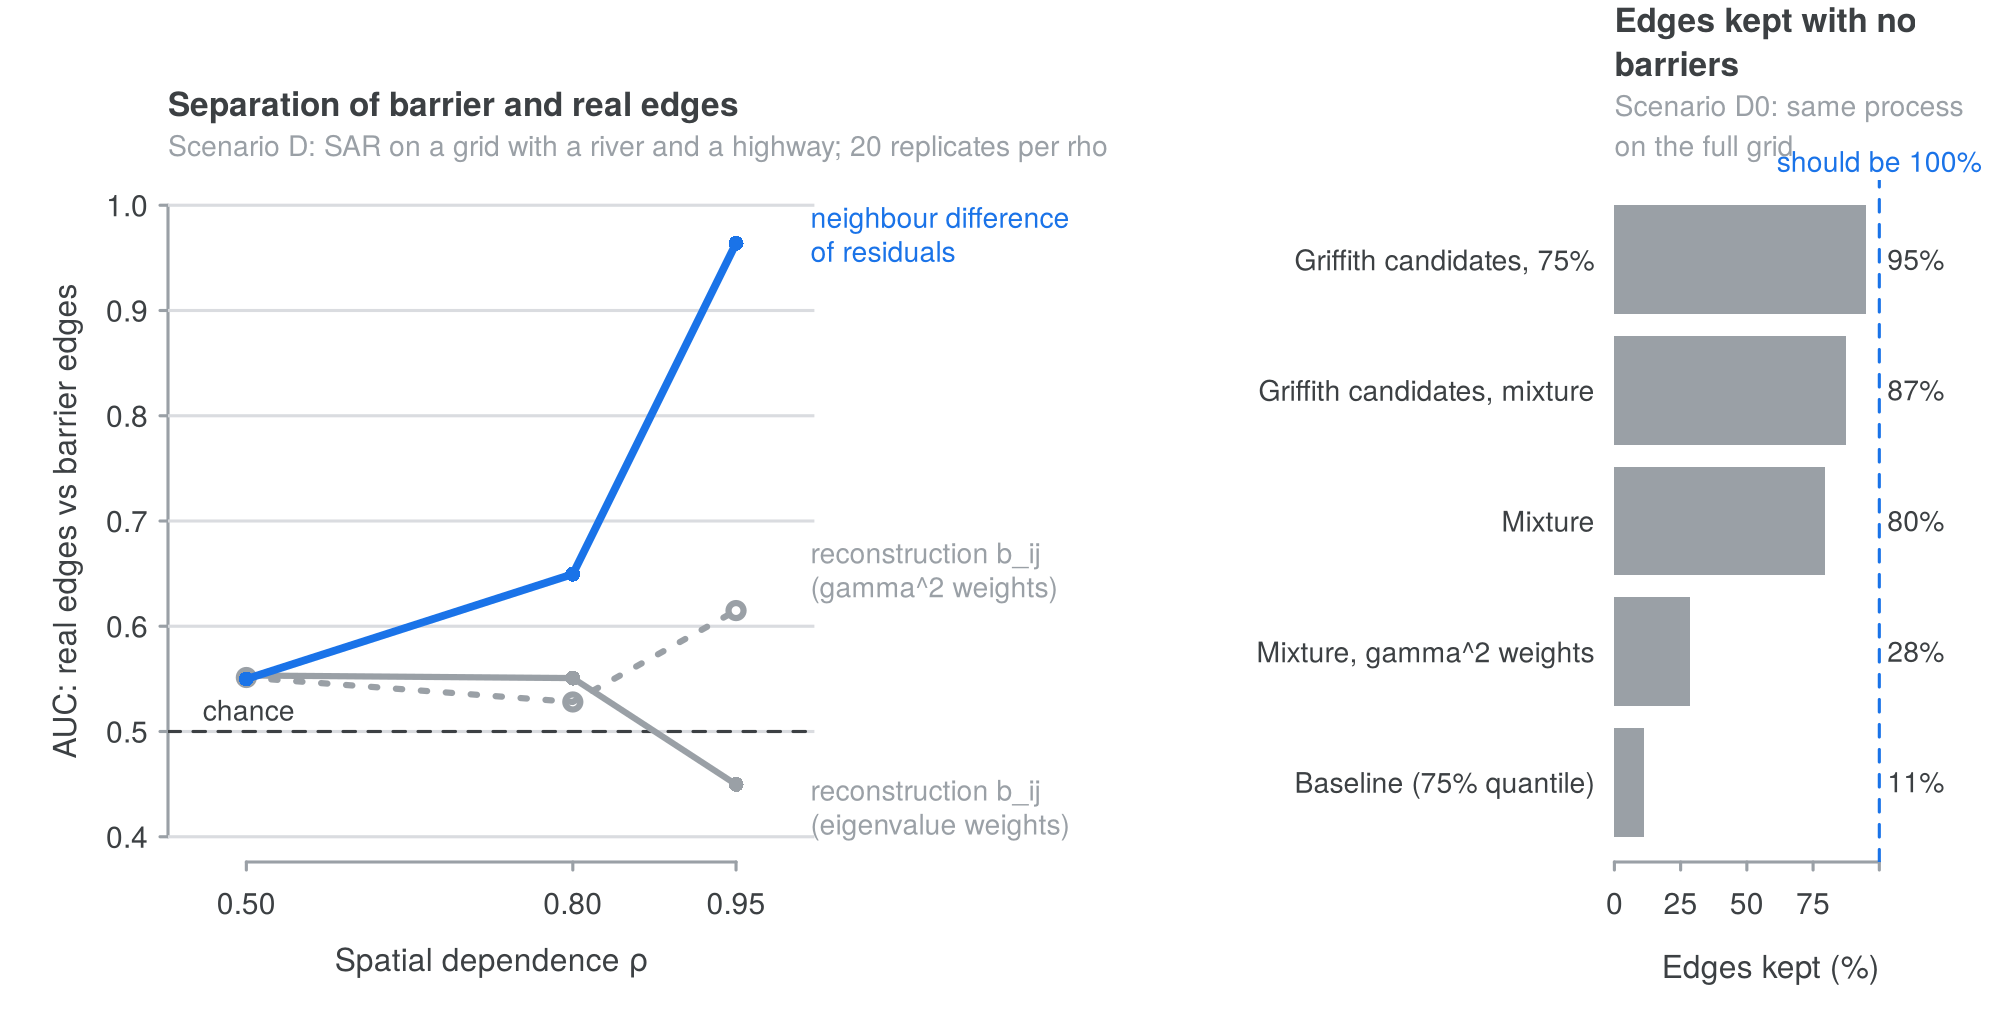
\includegraphics[width=\textwidth]{fig3_latent_graph}
\caption{Left: AUC for separating real edges from barrier edges in scenario D (20 replicates per $\rho$). Right: share of edges kept in scenario D0 by variant of the procedure.}
\label{fig:app-graph}
\end{figure}

\subsection{Conclusion}
\label{app:rec-conclusion}

In these simulations, no rounding rule increased the highest precision obtained without rounding by more than 0.01 (largest excess on the $20\times20$ grid; centrality among hot cells on the $40\times40$ grid). The reconstructed weights did not identify the edges removed by barriers, and most rounding rules removed most edges when no barrier was present. Ranking by centrality on the whole reconstructed graph selected cold cells in about half of the positions. The proposed procedure therefore uses the ESF step once, to estimate the spatial component $\hat f$ conditional on the covariates, and derives hot and cold zones from it on the contiguity graph $A$.

% Figures are read from ../simulation/figures/ (set in the preamble with
%     \graphicspath{{../simulation/figures/}}
% or copy the PNG files next to the .tex file).
% Packages used: graphicx, amsmath (both loaded by sn-jnl).
% Figures and tables are produced by simulation/04_iteration_figures.R from the
% results of simulation/01_ ... 06_*.R in the project repository.
% =====================================================================

\section{Iterative reconstruction of the spatial weights matrix}
\label{app:reconstruction}

This appendix describes an extension of the eigenvector spatial filtering (ESF) step that reconstructs a sparser spatial weights matrix from the selected eigenvectors and iterates the selection on the reconstructed graph. We evaluate it in simulation and explain why it is not part of the proposed procedure.

\subsection{The iterative reconstruction}
\label{app:rec-procedure}

Let $A$ be the $n\times n$ binary contiguity matrix of the study region, $Y$ the standardised counts per cell and $Z$ the standardised covariates. The procedure starts from $D^{(0)}=A$ and, at iteration $k$:

\begin{enumerate}
  \item computes the eigendecomposition $D^{(k)} = E\,\Delta\,E^\top$, with $\Delta=\mathrm{diag}(\delta_1,\dots,\delta_n)$, and selects a subset $S$ of eigenvectors with the MI-Lasso estimator, with penalty $\lambda=|z_0|^{-2}$ fixed from the standardised Moran's $I$ of the residuals of $Y$ on $Z$;
  \item reconstructs
  \begin{equation}
    B = E_S\,\Delta_S\,E_S^\top, \qquad b_{ij} = \sum_{s\in S}\delta_s\, e_s(i)\, e_s(j);
    \label{eq:app-B}
  \end{equation}
  \item applies a rounding rule: among the edges of $D^{(k)}$ with $b_{ij}>0$, it keeps those with $b_{ij}\ge\tau^{(k)}$, where $\tau^{(k)}$ is a threshold computed from these values, giving $D^{(k+1)} = D^{(k)}\circ\mathbf{1}\{B\ge\tau^{(k)}\}$;
  \item accepts $D^{(k+1)}$ if the post-Lasso residuals obtained with its eigenvectors show no spatial correlation (Moran's $I$ with $A$, level $0.05$), and stops otherwise or when $D^{(k+1)}=D^{(k)}$.
\end{enumerate}

Because each accepted step removes at least one edge, the procedure stops after at most as many iterations as $A$ has edges. Cells are then ranked by a ranking rule applied to the final graph.

We call \emph{baseline configuration} the procedure with all $n$ eigenvectors as candidates, eigenvalue weights in \eqref{eq:app-B}, the 75\% quantile of the positive $b_{ij}$ as threshold, and cells ranked by harmonic centrality on the final graph. Each variant below changes one element of the baseline.

\paragraph{Rounding rules.}
\emph{None} (all edges kept, $D=A$; no reconstruction);
\emph{quantile $q$} ($\tau$ = $q$-quantile of the positive $b_{ij}$ on the current edges, $q\in\{0.50, 0.75, 0.80, 0.90\}$);
\emph{mixture} (a two-component Gaussian mixture fitted to the positive $b_{ij}$; $\tau$ is the point between the two means where the weighted component densities are equal, and all edges are kept when the Bayesian information criterion selects one component);
\emph{permutation} (30 Freedman--Lane permutations of the residuals of $Y$ on $Z$; for each, the selection and \eqref{eq:app-B} are recomputed on the current graph, and $\tau$ is the 95th percentile of the pooled positive $b_{ij}$).

\paragraph{Ranking rules.}
Let $\hat f = E_S\hat\gamma_S$ be the fitted spatial component (centred), and call a cell \emph{hot} if $\hat f_i>0$ and \emph{cold} otherwise.
\emph{Centrality, whole graph}: harmonic centrality on the final graph, over all cells (baseline).
\emph{Centrality, hot cells}: harmonic centrality computed among hot cells only.
\emph{Largest excess}: hot cells ordered by $\hat f_i$.
\emph{Hot zones first}: connected groups of hot cells ordered by $\sum_{i}\hat f_i$; within a group, cells ordered by harmonic centrality.
Two benchmarks that do not use the graph are also reported: \emph{top counts} (cells ordered by $Y$) and \emph{top residuals} (cells ordered by the residuals of $Y$, or of $\log(Y+1)$, on $Z$).

\subsection{Simulation design}
\label{app:rec-design}

All scenarios use a $1000\times1000$ window divided into a regular grid with queen contiguity. Table~\ref{tab:app-scenarios} lists the scenarios.

\begin{table}[ht]
\centering
\caption{Simulated scenarios.}
\label{tab:app-scenarios}
\begin{tabular}{p{0.16\textwidth}p{0.50\textwidth}p{0.24\textwidth}}
\hline
Scenario & Data-generating process & Target \\
\hline
A: clusters & Three clusters: parents uniform in the window at least 100 units from the border; 500 offspring per parent, uniform in a disc of radius 100; 2000 additional uniform points. No covariate. & Cells inside the three discs \\
B: clusters and covariate & Scenario A plus 3000 points accepted with probability $\exp\{3(b(x)-1)\}$, where $b$ is a Gaussian surface (standard deviation 150) centred at least 300 units from every parent. The model receives $Z=(b,\ \varepsilon)$ at the cell centres, with $\varepsilon\sim N(0,1)$. & Cells inside the three discs, not the covariate area \\
D: barriers & $Y=\rho W Y + Z\beta + e$ on a $20\times20$ grid, with $W$ the row-standardised version of a graph $W^\ast\subset A$ in which a vertical line (one crossing left open) and a horizontal line on the left half remove 85 of the 1482 edges; $Z$ a linear gradient and noise, $\beta=(1,0)$, $\rho\in\{0.5,0.8,0.95\}$. & The 85 removed edges \\
D0: no barriers & As D with $W^\ast=A$. & No edge removed \\
\hline
\end{tabular}
\end{table}

Unless stated otherwise the grid has $20\times20$ cells (cell side 50) and the budget is the top 20 cells (5\%). For scenarios A and B, \emph{precision} is the share of the selected cells inside a true cluster disc. For scenarios D and D0, edges are classified as kept or removed, and we report the area under the ROC curve (AUC) of $b_{ij}$ for separating real from barrier edges, the share of edges kept, and Youden's $J$ = (share of barrier edges removed) + (share of real edges kept) $-\,1$, which is 0 for a classification unrelated to the barriers.

\subsection{Results}
\label{app:rec-results}

\paragraph{Sign of the reconstructed weights.}
Equation~\eqref{eq:app-B} is invariant to the sign of each eigenvector, since $e_s e_s^\top=(-e_s)(-e_s)^\top$. A positive $b_{ij}$ indicates that cells $i$ and $j$ lie on the same side of the selected spatial patterns, whether both have high or both have low counts. Under the baseline configuration, half of the 20 cells ranked highest in scenario B had $\hat f_i<0$, and precision was 0.28 in scenario A and 0.24 in scenario B (Fig.~\ref{fig:app-cold}). Ranking hot cells by $\hat f$ gave 1.00 and 0.96. Figure~\ref{fig:app-example} shows the successive graphs and the selected cells for one simulated map.

\begin{figure}[ht]
\centering
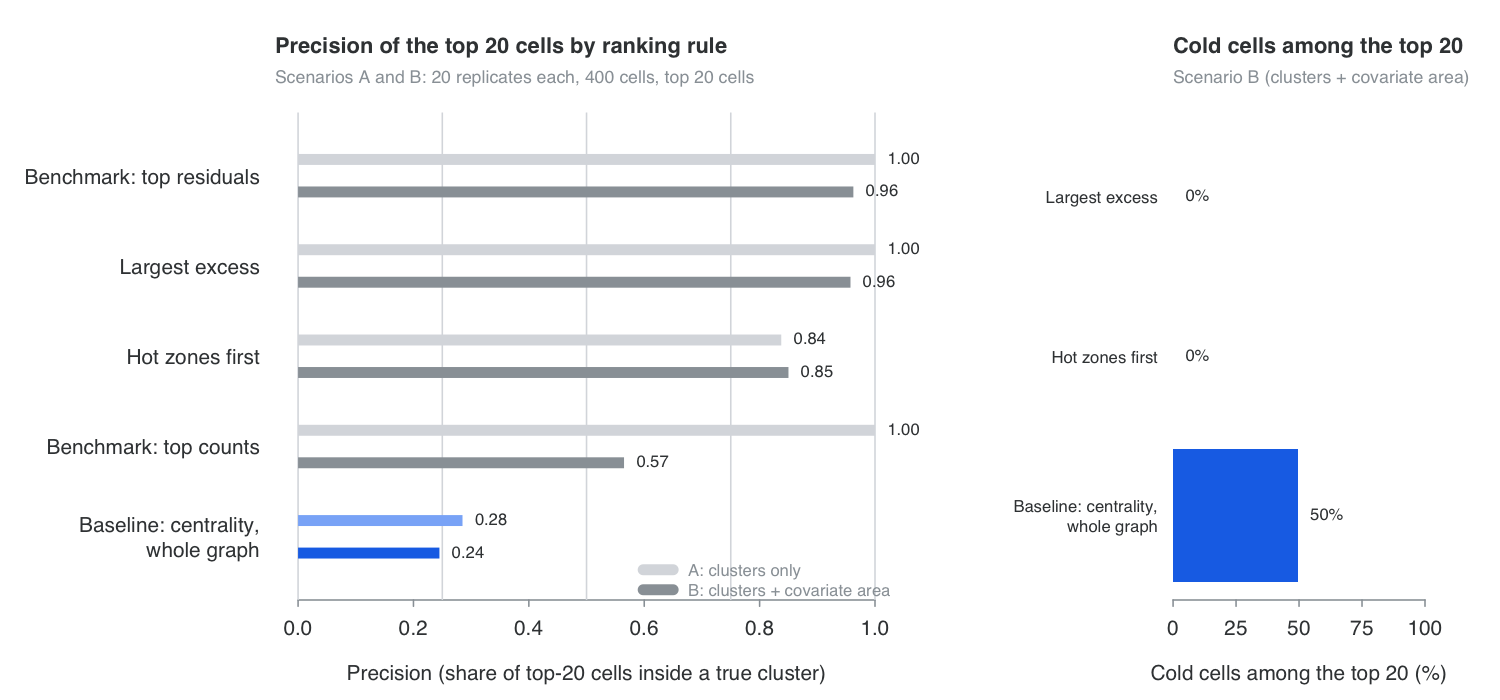
\includegraphics[width=\textwidth]{fig1_cold_zones}
\caption{Precision of the top 20 of 400 cells by ranking rule (scenarios A and B, 20 replicates each) and share of cold cells among them (scenario B). Baseline: harmonic centrality on the final graph.}
\label{fig:app-cold}
\end{figure}

\begin{figure}[ht]
\centering
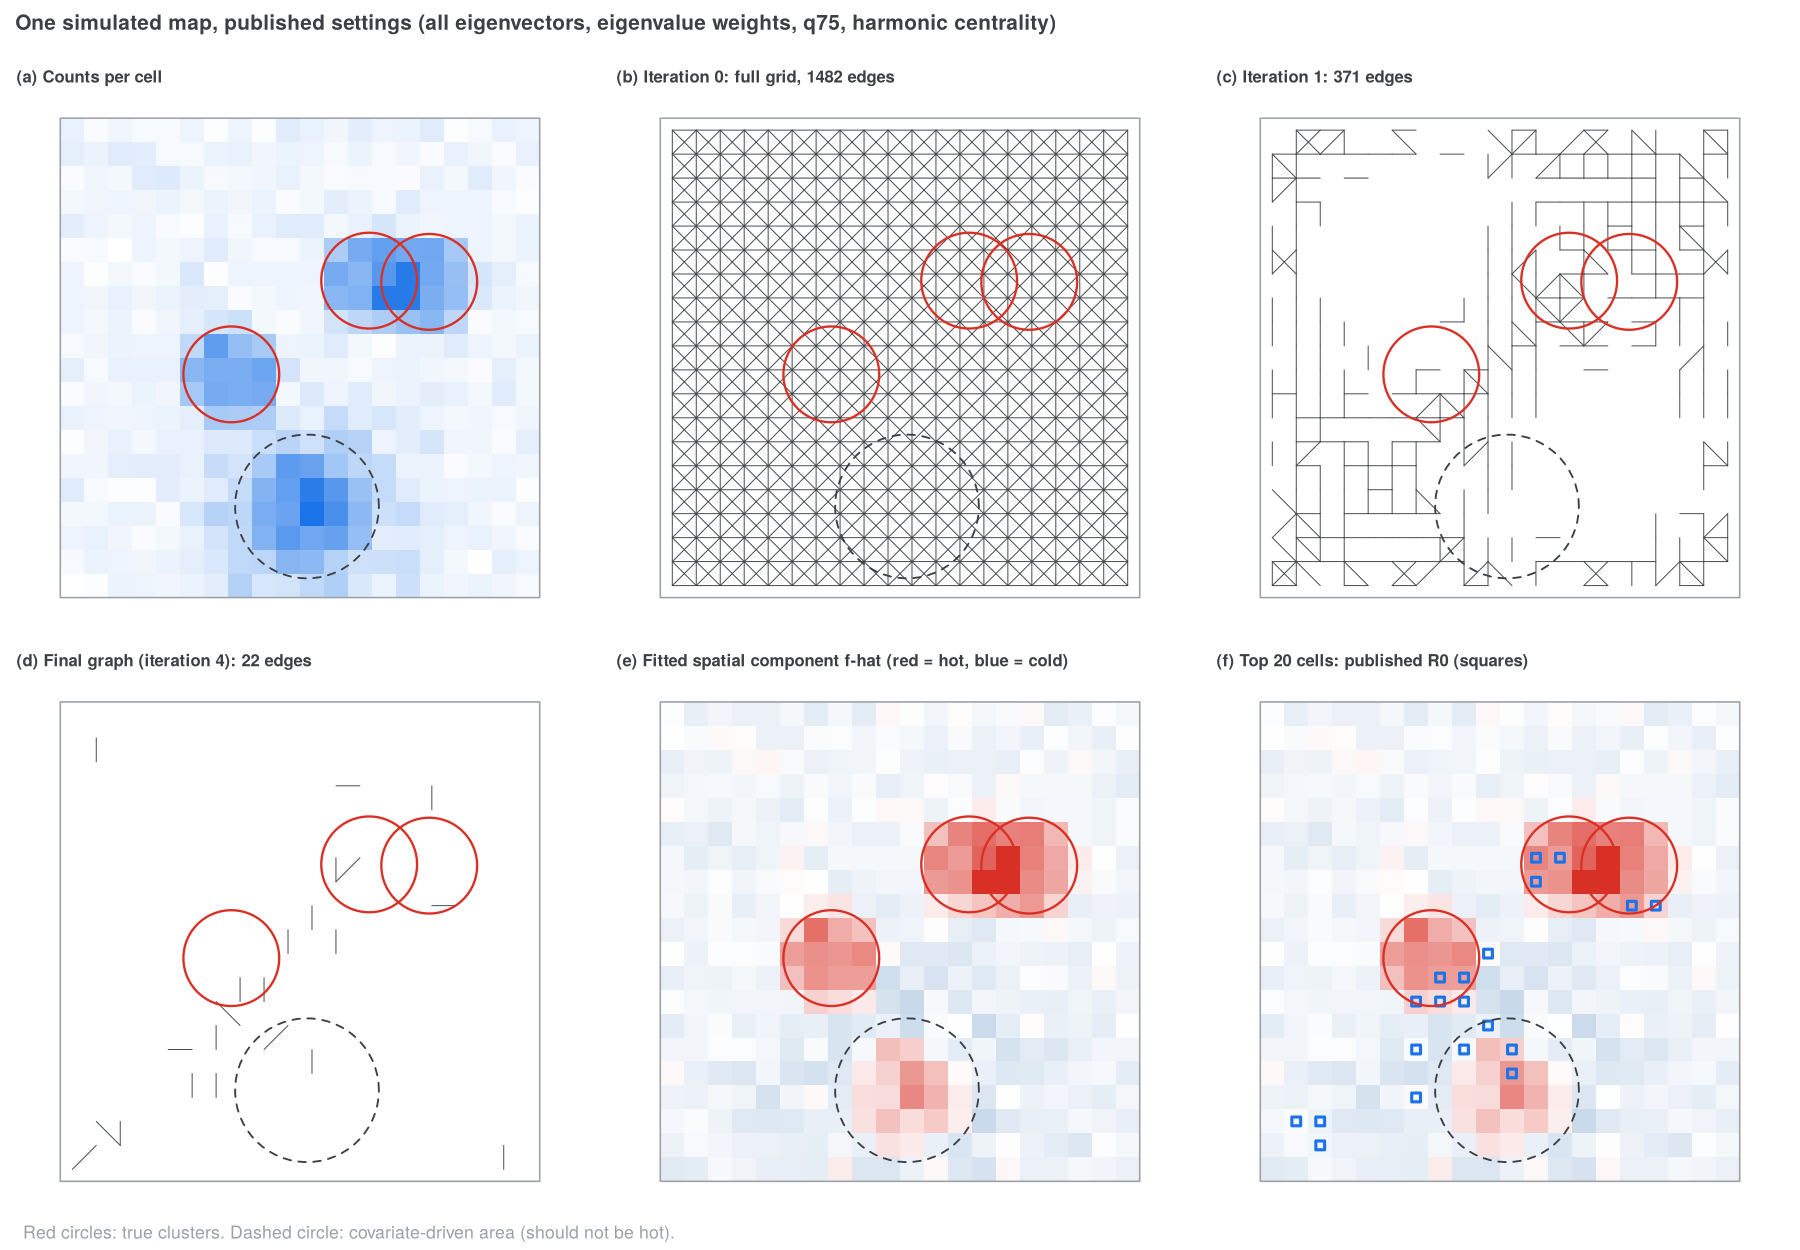
\includegraphics[width=\textwidth]{figS2_example_run}
\caption{One simulated map from scenario B under the baseline configuration. (a) Counts per cell. (b)--(d) Graph at iterations 0, 1 and at the last accepted iteration. (e) Fitted spatial component $\hat f$. (f) Top 20 cells under the baseline ranking. Circles: true clusters; dashed circle: covariate area.}
\label{fig:app-example}
\end{figure}

\paragraph{Effect of rounding and iteration on the selected cells.}
We compared rounding with the 75\% quantile against no rounding over 162 settings of scenario B: grids of $10\times10$, $20\times20$ and $40\times40$ cells, 50, 200 or 500 points per cluster, penalty exponents $a\in\{0.5,1,2\}$ in $\lambda=|z_0|^{-a}$, counts on the original or the $\log(Y+1)$ scale, and three ranking rules (10 replicates per setting). Iteration removed edges in 495 of 1620 runs (31\%); in the remaining runs the first reduced graph was rejected by the Moran test. In the runs where edges were removed, the change in precision was $+0.06$ (95\% CI $0.02$ to $0.10$) for centrality on the whole graph, $-0.01$ ($-0.03$ to $0.01$) for largest excess and $-0.06$ ($-0.11$ to $-0.01$) for hot zones first (Fig.~\ref{fig:app-iteration}).

\begin{figure}[ht]
\centering
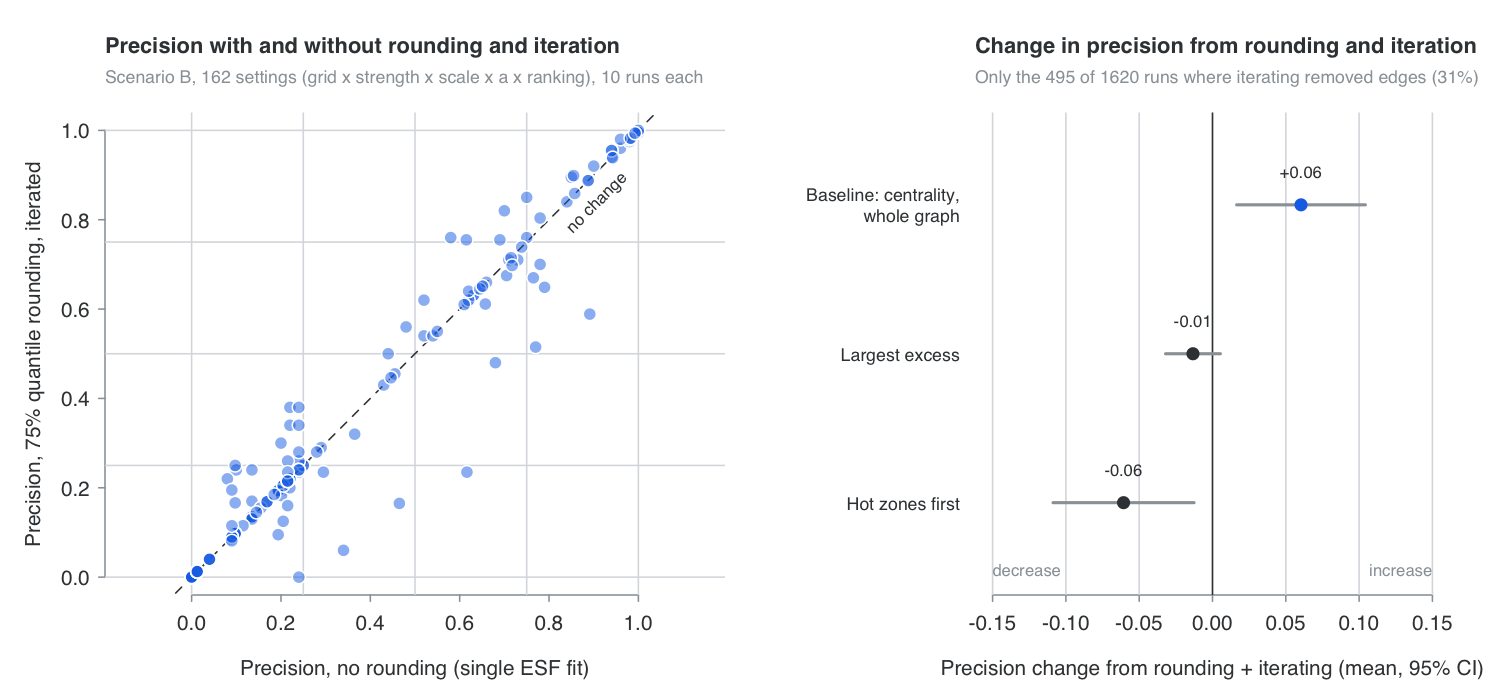
\includegraphics[width=\textwidth]{fig2_iteration_no_effect}
\caption{Left: precision with no rounding against precision with 75\% quantile rounding and iteration; each point is one setting (mean of 10 replicates). Right: change in precision in the runs where iteration removed edges (mean and 95\% confidence interval).}
\label{fig:app-iteration}
\end{figure}

\paragraph{Rounding rules.}
Table~\ref{tab:app-rounding} and Fig.~\ref{fig:app-rounding} compare the seven rounding rules with all other elements fixed at the baseline (scenarios A and B, 20 replicates each; scenarios D and D0, 20 replicates each). With the largest-excess ranking, precision was 1.00 in scenario A and 0.95--0.96 in scenario B for every rule, including no rounding. With hot zones first, the 80\% and 90\% quantiles and the permutation rule gave about 0.10 more than no rounding, and remained below the largest-excess ranking. With the baseline ranking, precision ranged from 0.10 to 0.37. In scenario D0 every rule except the mixture removed between 90\% and 97\% of the edges.

\begin{table}[ht]
\centering
\caption{Precision of the top 20 cells (scenario A / scenario B) by rounding rule and ranking rule, and share of edges kept in scenario D0. Mean of 20 replicates.}
\label{tab:app-rounding}
\small\setlength{\tabcolsep}{4pt}
\begin{tabular}{lcccc}
\hline
Rounding rule & Largest excess & Hot zones first & Centrality, & Edges kept \\
 & & & whole graph & (D0) \\
\hline
None            & 1.00 / 0.95 & 0.85 / 0.76 & 0.13 / 0.10 & 100\% \\
50\% quantile   & 1.00 / 0.95 & 0.81 / 0.71 & 0.32 / 0.37 & 6\% \\
75\% quantile (baseline) & 1.00 / 0.95 & 0.84 / 0.84 & 0.22 / 0.29 & 8\% \\
80\% quantile   & 1.00 / 0.95 & 0.89 / 0.90 & 0.19 / 0.31 & 3\% \\
90\% quantile   & 1.00 / 0.95 & 0.91 / 0.91 & 0.26 / 0.32 & 10\% \\
Mixture         & 1.00 / 0.96 & 0.80 / 0.78 & 0.26 / 0.31 & 76\% \\
Permutation     & 1.00 / 0.95 & 0.90 / 0.91 & 0.23 / 0.37 & 10\% \\
\hline
\end{tabular}
\end{table}

\begin{figure}[ht]
\centering
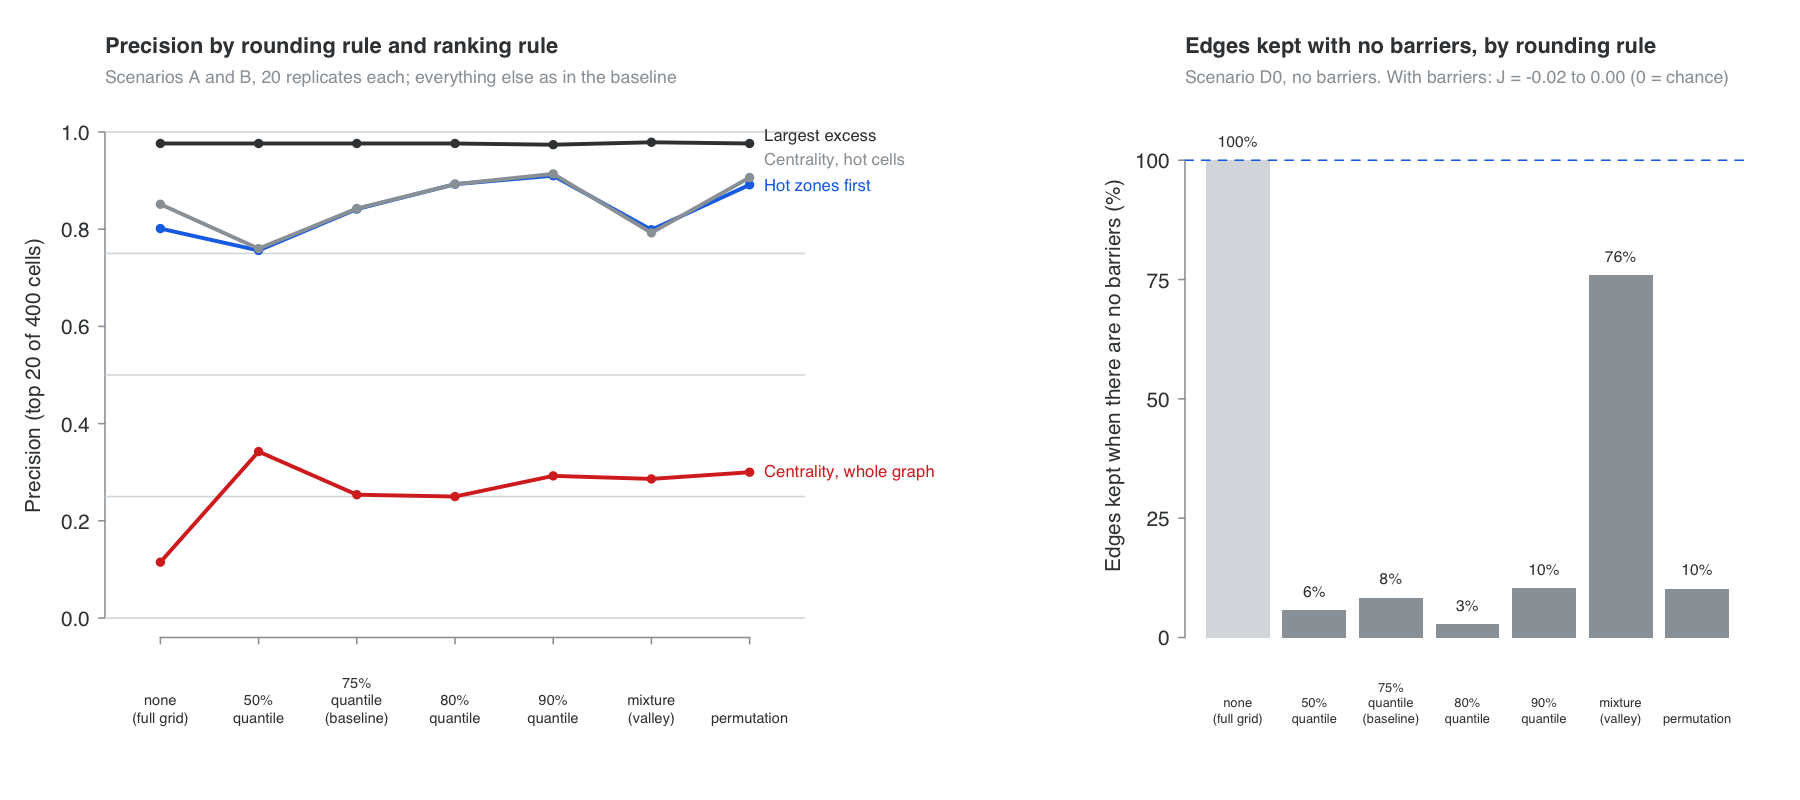
\includegraphics[width=\textwidth]{fig4_rounding_rules}
\caption{Left: precision of the top 20 of 400 cells by rounding rule and ranking rule (scenarios A and B pooled, 20 replicates each). Right: share of edges kept in scenario D0, where no edge should be removed. Rules: none (full grid), q50--q90 (quantile of the positive $b_{ij}$; q75 is the baseline), mix (two-component mixture), perm (permutation).}
\label{fig:app-rounding}
\end{figure}

\paragraph{Fine grid with weak clusters.}
On a $40\times40$ grid (cell side 25) with 50 or 200 points per cluster, scenario B, budget of 80 cells, 10 replicates, the rankings that use hot cells and connectivity reached, with no rounding, a precision of 0.44--0.48 (50 points) and 0.81--0.89 (200 points), against 0.29 and 0.80 for top residuals on the log scale. Rounding reduced the precision of hot zones first by 0.24 and 0.25 (75\% quantile), 0.18 and 0.17 (90\% quantile) and 0.06 and 0.10 (permutation) (Fig.~\ref{fig:app-finegrid}).

\begin{figure}[ht]
\centering
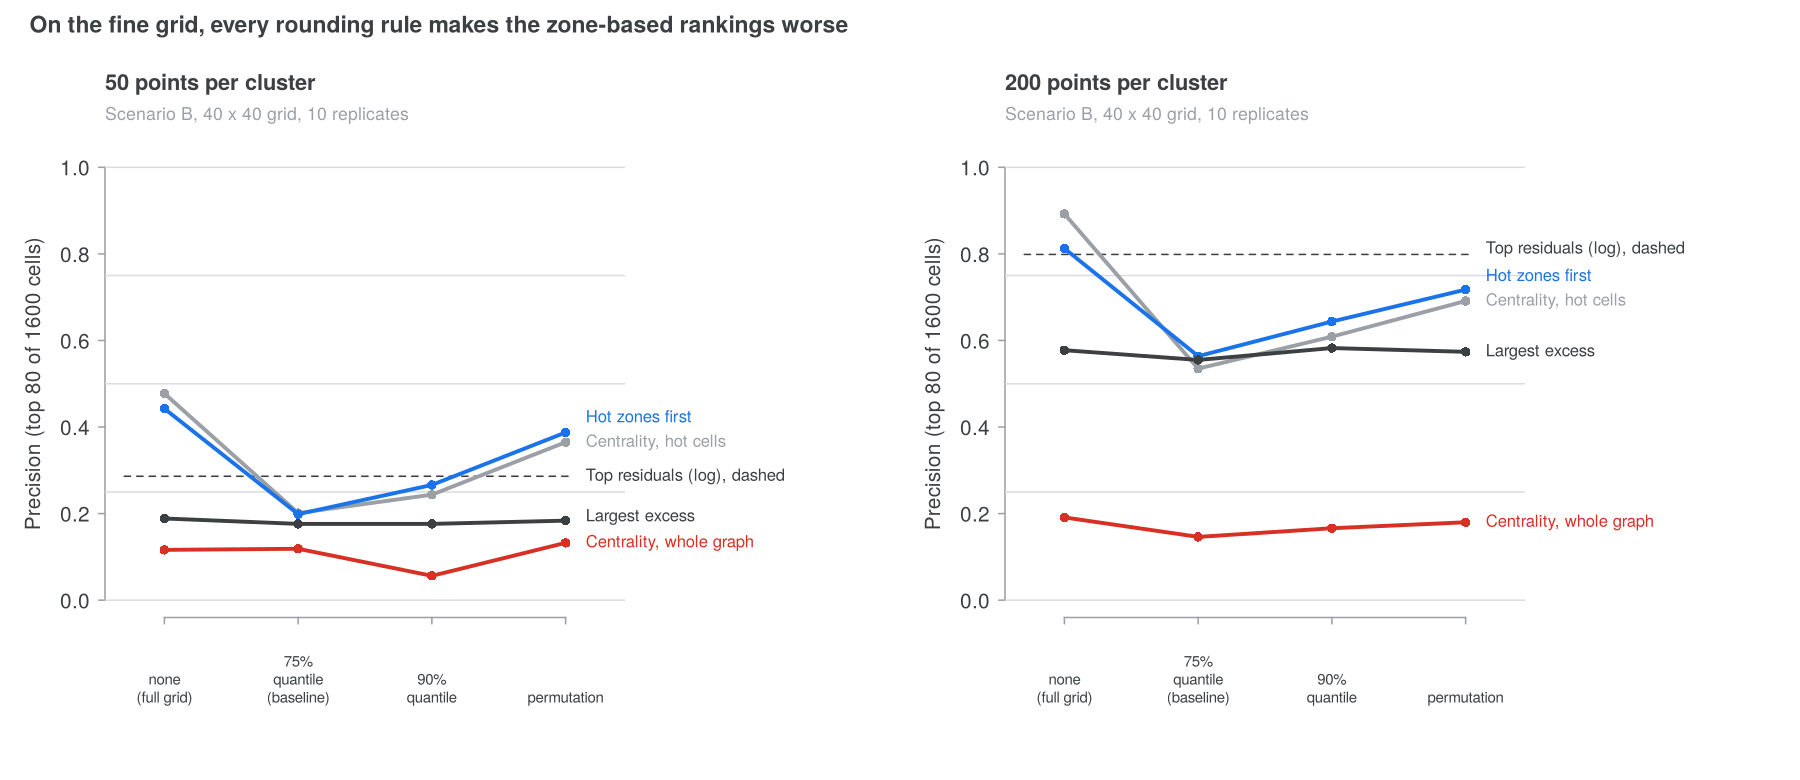
\includegraphics[width=\textwidth]{fig5_fine_grid}
\caption{Precision of the top 80 of 1600 cells by rounding rule and ranking rule on a $40\times40$ grid (scenario B, 10 replicates per panel). Dashed line: top residuals of $\log(Y+1)$ on $Z$. Rule labels as in Figure~\ref{fig:app-rounding}.}
\label{fig:app-finegrid}
\end{figure}

\paragraph{Recovery of a known graph.}
In scenario D, the AUC of $b_{ij}$ for separating real from barrier edges was 0.55, 0.55 and 0.45 for $\rho=0.5$, $0.8$ and $0.95$ with eigenvalue weights, and 0.55, 0.53 and 0.61 with squared coefficients $\hat\gamma_s^2$ as weights. The absolute difference between the residuals of neighbouring cells, $|e_i-e_j|$, gave 0.55, 0.65 and 0.96 (Fig.~\ref{fig:app-graph}). After the full procedure, Youden's $J$ ranged from $-0.02$ to $0.00$ across rounding rules. With 130--300 of 400 eigenvectors selected, $B$ differs from $A$ by a small number of patterns with global support, while a barrier is a local discontinuity.

\begin{figure}[ht]
\centering
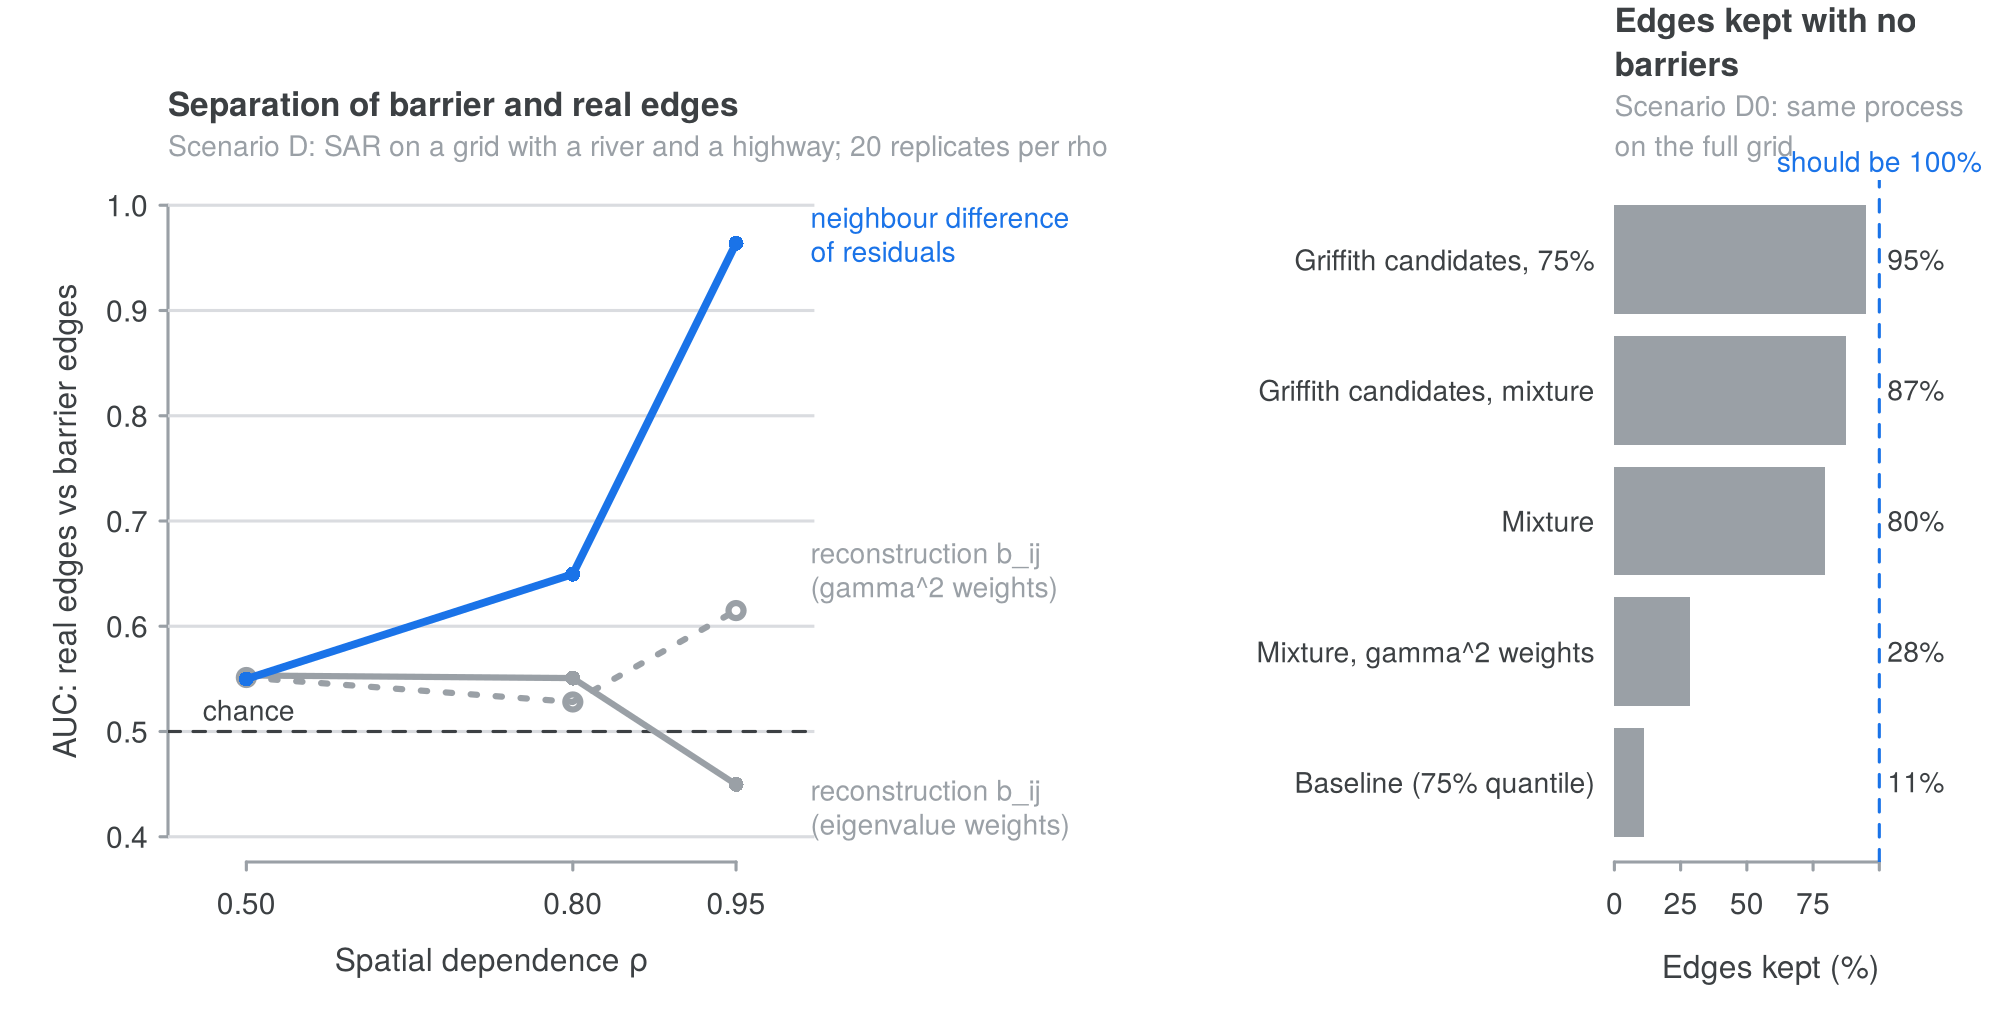
\includegraphics[width=\textwidth]{fig3_latent_graph}
\caption{Left: AUC for separating real edges from barrier edges in scenario D (20 replicates per $\rho$). Right: share of edges kept in scenario D0 by variant of the procedure.}
\label{fig:app-graph}
\end{figure}

\subsection{Conclusion}
\label{app:rec-conclusion}

In these simulations, no rounding rule increased the highest precision obtained without rounding by more than 0.01 (largest excess on the $20\times20$ grid; centrality among hot cells on the $40\times40$ grid). The reconstructed weights did not identify the edges removed by barriers, and most rounding rules removed most edges when no barrier was present. Ranking by centrality on the whole reconstructed graph selected cold cells in about half of the positions. The proposed procedure therefore uses the ESF step once, to estimate the spatial component $\hat f$ conditional on the covariates, and derives hot and cold zones from it on the contiguity graph $A$.

% Figures are read from ../simulation/figures/ (set in the preamble with
%     \graphicspath{{../simulation/figures/}}
% or copy the PNG files next to the .tex file).
% Packages used: graphicx, amsmath (both loaded by sn-jnl).
% Figures and tables are produced by simulation/04_iteration_figures.R from the
% results of simulation/01_ ... 06_*.R in the project repository.
% =====================================================================

\section{Iterative reconstruction of the spatial weights matrix}
\label{app:reconstruction}

This appendix describes an extension of the eigenvector spatial filtering (ESF) step that reconstructs a sparser spatial weights matrix from the selected eigenvectors and iterates the selection on the reconstructed graph. We evaluate it in simulation and explain why it is not part of the proposed procedure.

\subsection{The iterative reconstruction}
\label{app:rec-procedure}

Let $A$ be the $n\times n$ binary contiguity matrix of the study region, $Y$ the standardised counts per cell and $Z$ the standardised covariates. The procedure starts from $D^{(0)}=A$ and, at iteration $k$:

\begin{enumerate}
  \item computes the eigendecomposition $D^{(k)} = E\,\Delta\,E^\top$, with $\Delta=\mathrm{diag}(\delta_1,\dots,\delta_n)$, and selects a subset $S$ of eigenvectors with the MI-Lasso estimator, with penalty $\lambda=|z_0|^{-2}$ fixed from the standardised Moran's $I$ of the residuals of $Y$ on $Z$;
  \item reconstructs
  \begin{equation}
    B = E_S\,\Delta_S\,E_S^\top, \qquad b_{ij} = \sum_{s\in S}\delta_s\, e_s(i)\, e_s(j);
    \label{eq:app-B}
  \end{equation}
  \item applies a rounding rule: among the edges of $D^{(k)}$ with $b_{ij}>0$, it keeps those with $b_{ij}\ge\tau^{(k)}$, where $\tau^{(k)}$ is a threshold computed from these values, giving $D^{(k+1)} = D^{(k)}\circ\mathbf{1}\{B\ge\tau^{(k)}\}$;
  \item accepts $D^{(k+1)}$ if the post-Lasso residuals obtained with its eigenvectors show no spatial correlation (Moran's $I$ with $A$, level $0.05$), and stops otherwise or when $D^{(k+1)}=D^{(k)}$.
\end{enumerate}

Because each accepted step removes at least one edge, the procedure stops after at most as many iterations as $A$ has edges. Cells are then ranked by a ranking rule applied to the final graph.

We call \emph{baseline configuration} the procedure with all $n$ eigenvectors as candidates, eigenvalue weights in \eqref{eq:app-B}, the 75\% quantile of the positive $b_{ij}$ as threshold, and cells ranked by harmonic centrality on the final graph. Each variant below changes one element of the baseline.

\paragraph{Rounding rules.}
\emph{None} (all edges kept, $D=A$; no reconstruction);
\emph{quantile $q$} ($\tau$ = $q$-quantile of the positive $b_{ij}$ on the current edges, $q\in\{0.50, 0.75, 0.80, 0.90\}$);
\emph{mixture} (a two-component Gaussian mixture fitted to the positive $b_{ij}$; $\tau$ is the point between the two means where the weighted component densities are equal, and all edges are kept when the Bayesian information criterion selects one component);
\emph{permutation} (30 Freedman--Lane permutations of the residuals of $Y$ on $Z$; for each, the selection and \eqref{eq:app-B} are recomputed on the current graph, and $\tau$ is the 95th percentile of the pooled positive $b_{ij}$).

\paragraph{Ranking rules.}
Let $\hat f = E_S\hat\gamma_S$ be the fitted spatial component (centred), and call a cell \emph{hot} if $\hat f_i>0$ and \emph{cold} otherwise.
\emph{Centrality, whole graph}: harmonic centrality on the final graph, over all cells (baseline).
\emph{Centrality, hot cells}: harmonic centrality computed among hot cells only.
\emph{Largest excess}: hot cells ordered by $\hat f_i$.
\emph{Hot zones first}: connected groups of hot cells ordered by $\sum_{i}\hat f_i$; within a group, cells ordered by harmonic centrality.
Two benchmarks that do not use the graph are also reported: \emph{top counts} (cells ordered by $Y$) and \emph{top residuals} (cells ordered by the residuals of $Y$, or of $\log(Y+1)$, on $Z$).

\subsection{Simulation design}
\label{app:rec-design}

All scenarios use a $1000\times1000$ window divided into a regular grid with queen contiguity. Table~\ref{tab:app-scenarios} lists the scenarios.

\begin{table}[ht]
\centering
\caption{Simulated scenarios.}
\label{tab:app-scenarios}
\begin{tabular}{p{0.16\textwidth}p{0.50\textwidth}p{0.24\textwidth}}
\hline
Scenario & Data-generating process & Target \\
\hline
A: clusters & Three clusters: parents uniform in the window at least 100 units from the border; 500 offspring per parent, uniform in a disc of radius 100; 2000 additional uniform points. No covariate. & Cells inside the three discs \\
B: clusters and covariate & Scenario A plus 3000 points accepted with probability $\exp\{3(b(x)-1)\}$, where $b$ is a Gaussian surface (standard deviation 150) centred at least 300 units from every parent. The model receives $Z=(b,\ \varepsilon)$ at the cell centres, with $\varepsilon\sim N(0,1)$. & Cells inside the three discs, not the covariate area \\
D: barriers & $Y=\rho W Y + Z\beta + e$ on a $20\times20$ grid, with $W$ the row-standardised version of a graph $W^\ast\subset A$ in which a vertical line (one crossing left open) and a horizontal line on the left half remove 85 of the 1482 edges; $Z$ a linear gradient and noise, $\beta=(1,0)$, $\rho\in\{0.5,0.8,0.95\}$. & The 85 removed edges \\
D0: no barriers & As D with $W^\ast=A$. & No edge removed \\
\hline
\end{tabular}
\end{table}

Unless stated otherwise the grid has $20\times20$ cells (cell side 50) and the budget is the top 20 cells (5\%). For scenarios A and B, \emph{precision} is the share of the selected cells inside a true cluster disc. For scenarios D and D0, edges are classified as kept or removed, and we report the area under the ROC curve (AUC) of $b_{ij}$ for separating real from barrier edges, the share of edges kept, and Youden's $J$ = (share of barrier edges removed) + (share of real edges kept) $-\,1$, which is 0 for a classification unrelated to the barriers.

\subsection{Results}
\label{app:rec-results}

\paragraph{Sign of the reconstructed weights.}
Equation~\eqref{eq:app-B} is invariant to the sign of each eigenvector, since $e_s e_s^\top=(-e_s)(-e_s)^\top$. A positive $b_{ij}$ indicates that cells $i$ and $j$ lie on the same side of the selected spatial patterns, whether both have high or both have low counts. Under the baseline configuration, half of the 20 cells ranked highest in scenario B had $\hat f_i<0$, and precision was 0.28 in scenario A and 0.24 in scenario B (Fig.~\ref{fig:app-cold}). Ranking hot cells by $\hat f$ gave 1.00 and 0.96. Figure~\ref{fig:app-example} shows the successive graphs and the selected cells for one simulated map.

\begin{figure}[ht]
\centering
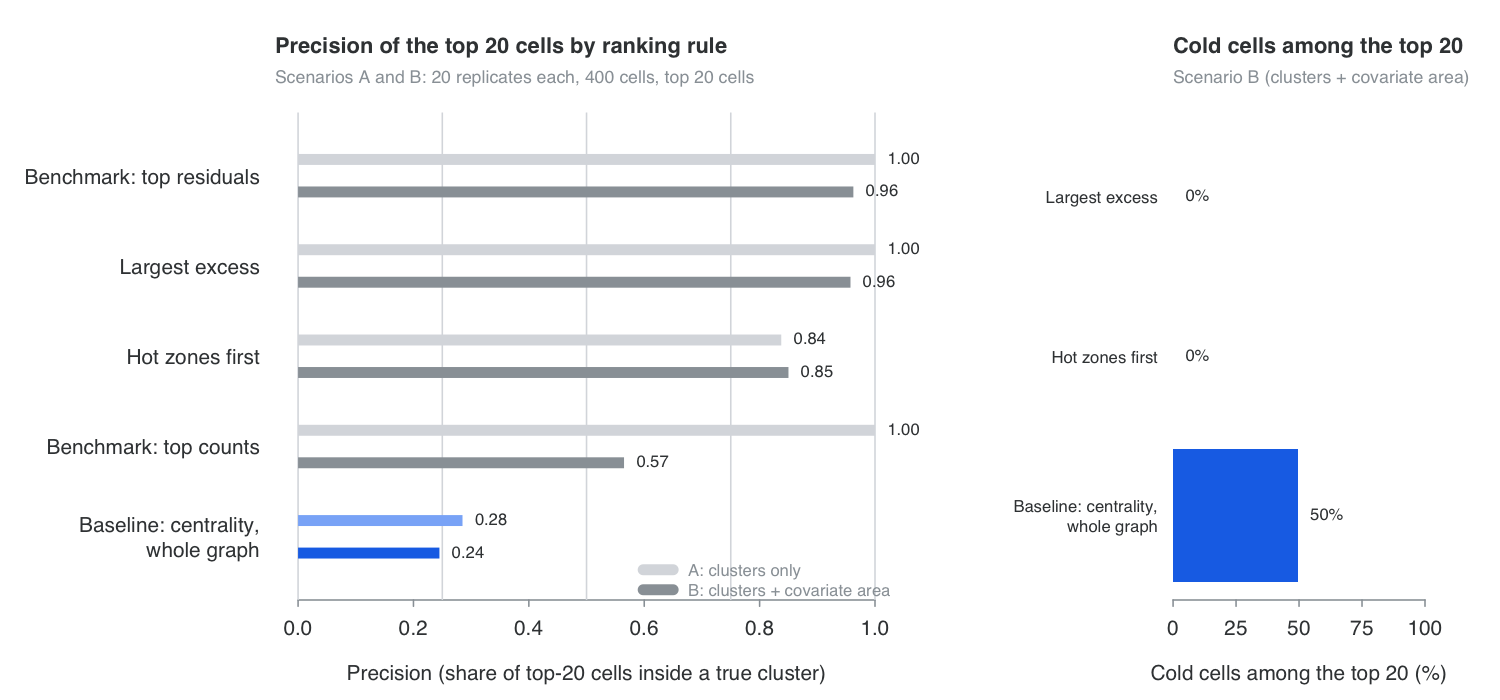
\includegraphics[width=\textwidth]{fig1_cold_zones}
\caption{Precision of the top 20 of 400 cells by ranking rule (scenarios A and B, 20 replicates each) and share of cold cells among them (scenario B). Baseline: harmonic centrality on the final graph.}
\label{fig:app-cold}
\end{figure}

\begin{figure}[ht]
\centering
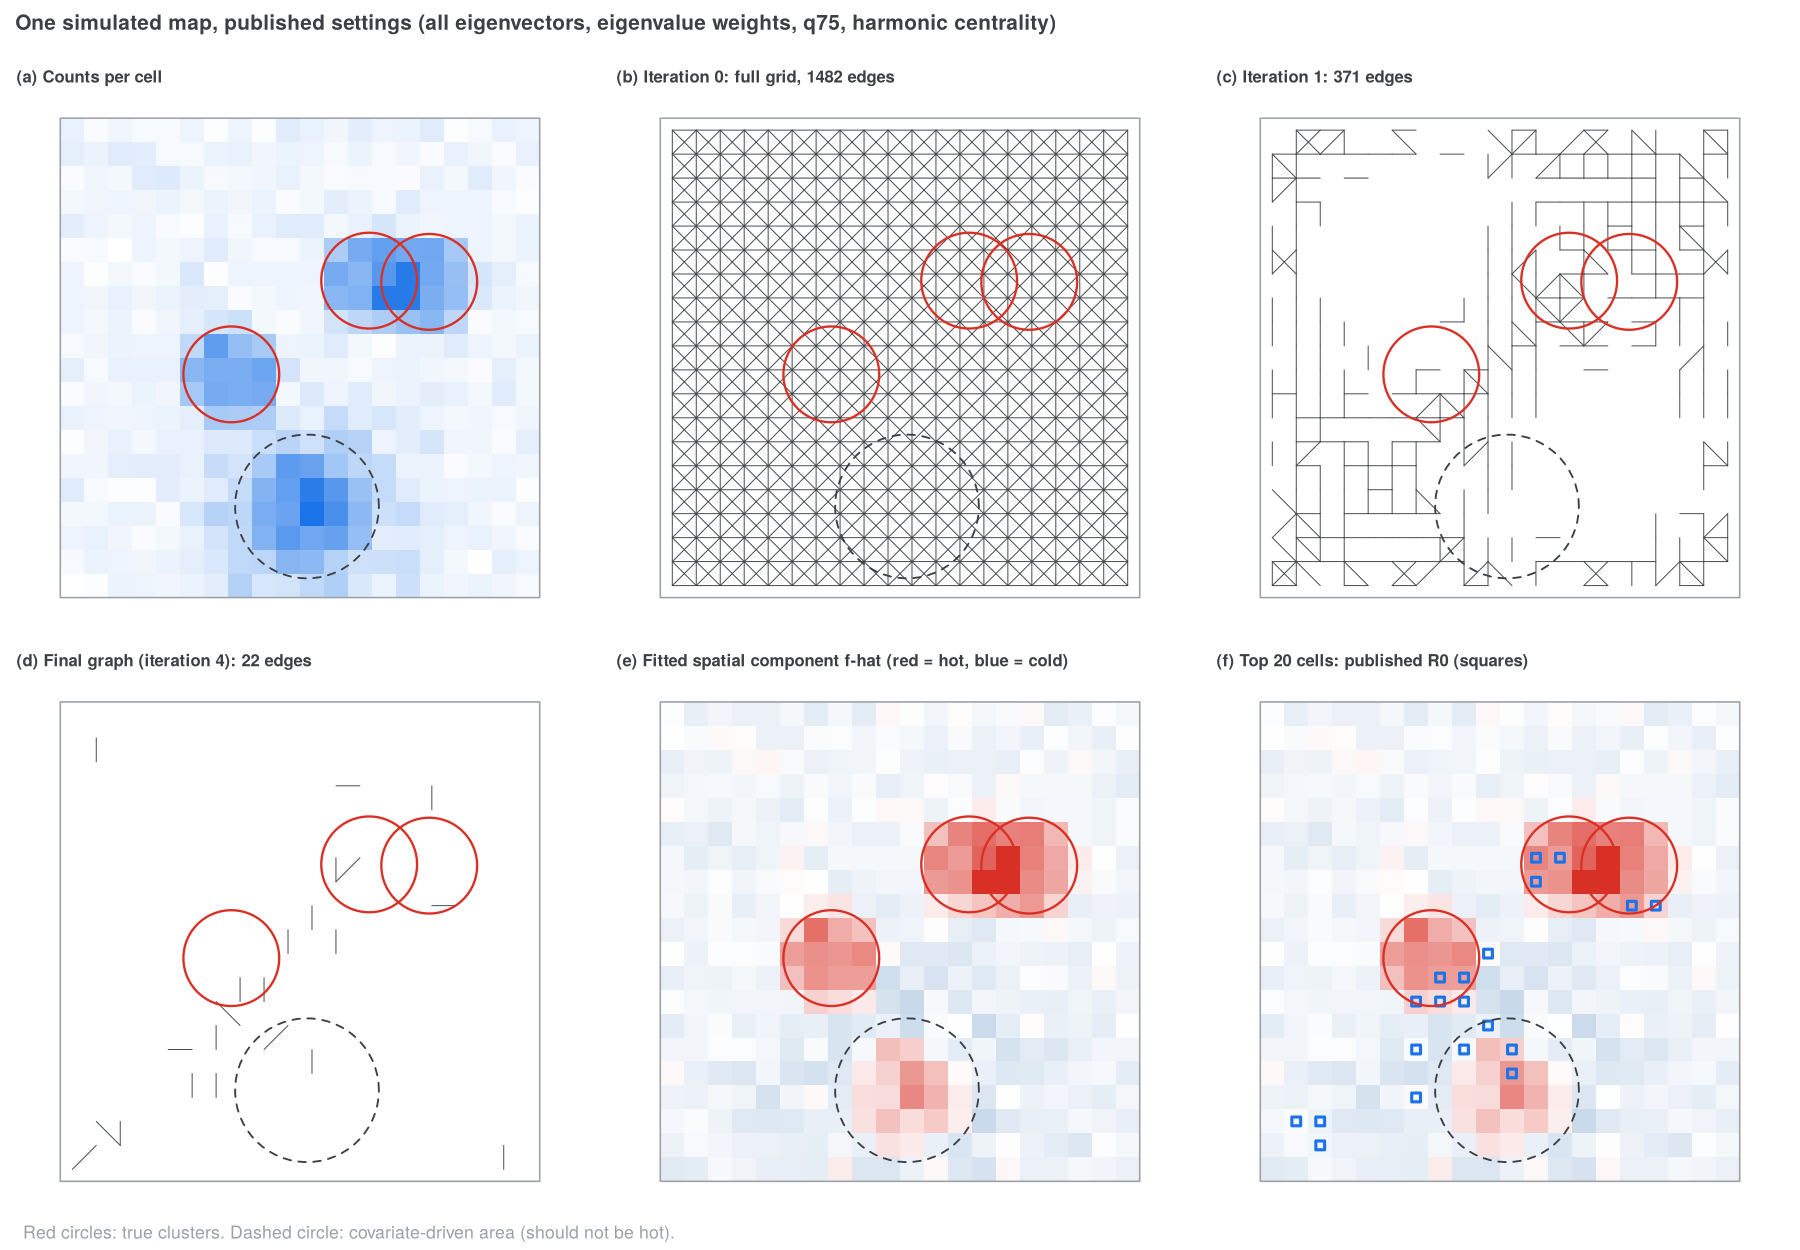
\includegraphics[width=\textwidth]{figS2_example_run}
\caption{One simulated map from scenario B under the baseline configuration. (a) Counts per cell. (b)--(d) Graph at iterations 0, 1 and at the last accepted iteration. (e) Fitted spatial component $\hat f$. (f) Top 20 cells under the baseline ranking. Circles: true clusters; dashed circle: covariate area.}
\label{fig:app-example}
\end{figure}

\paragraph{Effect of rounding and iteration on the selected cells.}
We compared rounding with the 75\% quantile against no rounding over 162 settings of scenario B: grids of $10\times10$, $20\times20$ and $40\times40$ cells, 50, 200 or 500 points per cluster, penalty exponents $a\in\{0.5,1,2\}$ in $\lambda=|z_0|^{-a}$, counts on the original or the $\log(Y+1)$ scale, and three ranking rules (10 replicates per setting). Iteration removed edges in 495 of 1620 runs (31\%); in the remaining runs the first reduced graph was rejected by the Moran test. In the runs where edges were removed, the change in precision was $+0.06$ (95\% CI $0.02$ to $0.10$) for centrality on the whole graph, $-0.01$ ($-0.03$ to $0.01$) for largest excess and $-0.06$ ($-0.11$ to $-0.01$) for hot zones first (Fig.~\ref{fig:app-iteration}).

\begin{figure}[ht]
\centering
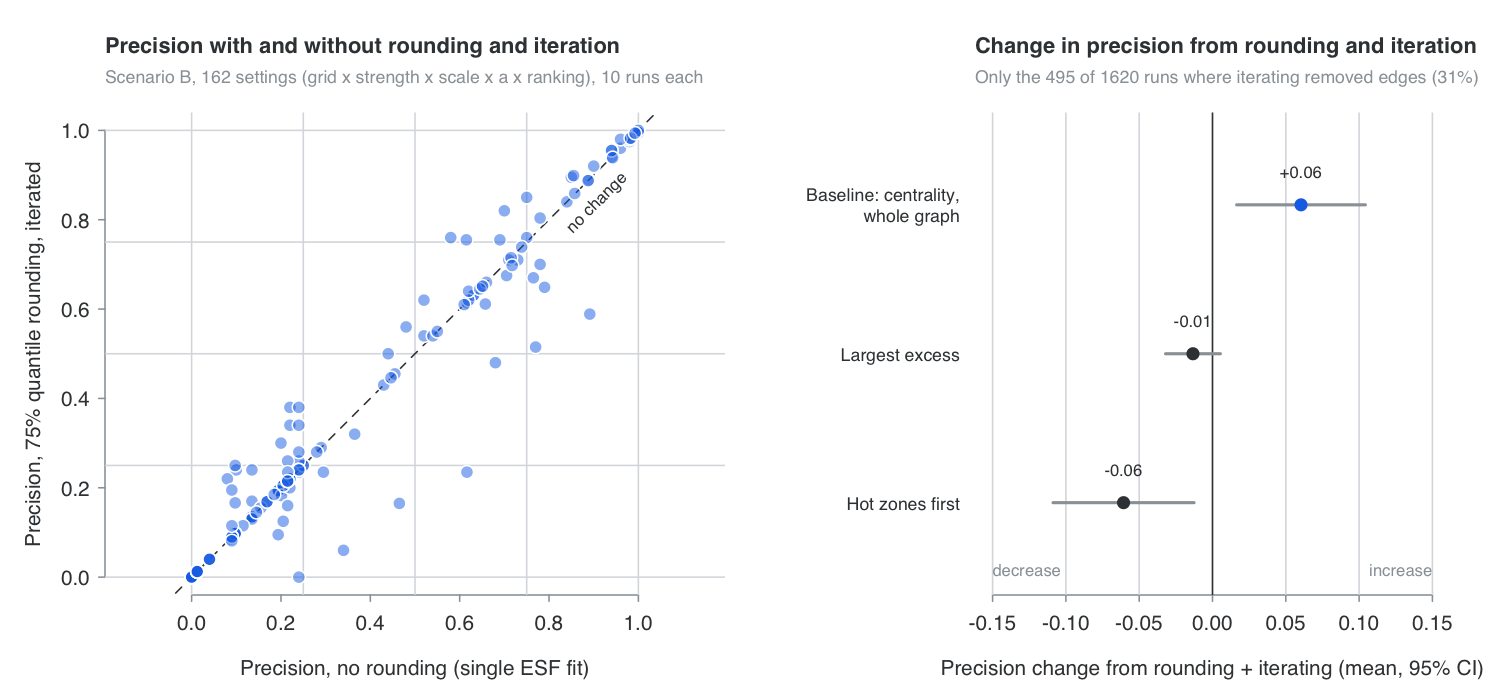
\includegraphics[width=\textwidth]{fig2_iteration_no_effect}
\caption{Left: precision with no rounding against precision with 75\% quantile rounding and iteration; each point is one setting (mean of 10 replicates). Right: change in precision in the runs where iteration removed edges (mean and 95\% confidence interval).}
\label{fig:app-iteration}
\end{figure}

\paragraph{Rounding rules.}
Table~\ref{tab:app-rounding} and Fig.~\ref{fig:app-rounding} compare the seven rounding rules with all other elements fixed at the baseline (scenarios A and B, 20 replicates each; scenarios D and D0, 20 replicates each). With the largest-excess ranking, precision was 1.00 in scenario A and 0.95--0.96 in scenario B for every rule, including no rounding. With hot zones first, the 80\% and 90\% quantiles and the permutation rule gave about 0.10 more than no rounding, and remained below the largest-excess ranking. With the baseline ranking, precision ranged from 0.10 to 0.37. In scenario D0 every rule except the mixture removed between 90\% and 97\% of the edges.

\begin{table}[ht]
\centering
\caption{Precision of the top 20 cells (scenario A / scenario B) by rounding rule and ranking rule, and share of edges kept in scenario D0. Mean of 20 replicates.}
\label{tab:app-rounding}
\small\setlength{\tabcolsep}{4pt}
\begin{tabular}{lcccc}
\hline
Rounding rule & Largest excess & Hot zones first & Centrality, & Edges kept \\
 & & & whole graph & (D0) \\
\hline
None            & 1.00 / 0.95 & 0.85 / 0.76 & 0.13 / 0.10 & 100\% \\
50\% quantile   & 1.00 / 0.95 & 0.81 / 0.71 & 0.32 / 0.37 & 6\% \\
75\% quantile (baseline) & 1.00 / 0.95 & 0.84 / 0.84 & 0.22 / 0.29 & 8\% \\
80\% quantile   & 1.00 / 0.95 & 0.89 / 0.90 & 0.19 / 0.31 & 3\% \\
90\% quantile   & 1.00 / 0.95 & 0.91 / 0.91 & 0.26 / 0.32 & 10\% \\
Mixture         & 1.00 / 0.96 & 0.80 / 0.78 & 0.26 / 0.31 & 76\% \\
Permutation     & 1.00 / 0.95 & 0.90 / 0.91 & 0.23 / 0.37 & 10\% \\
\hline
\end{tabular}
\end{table}

\begin{figure}[ht]
\centering
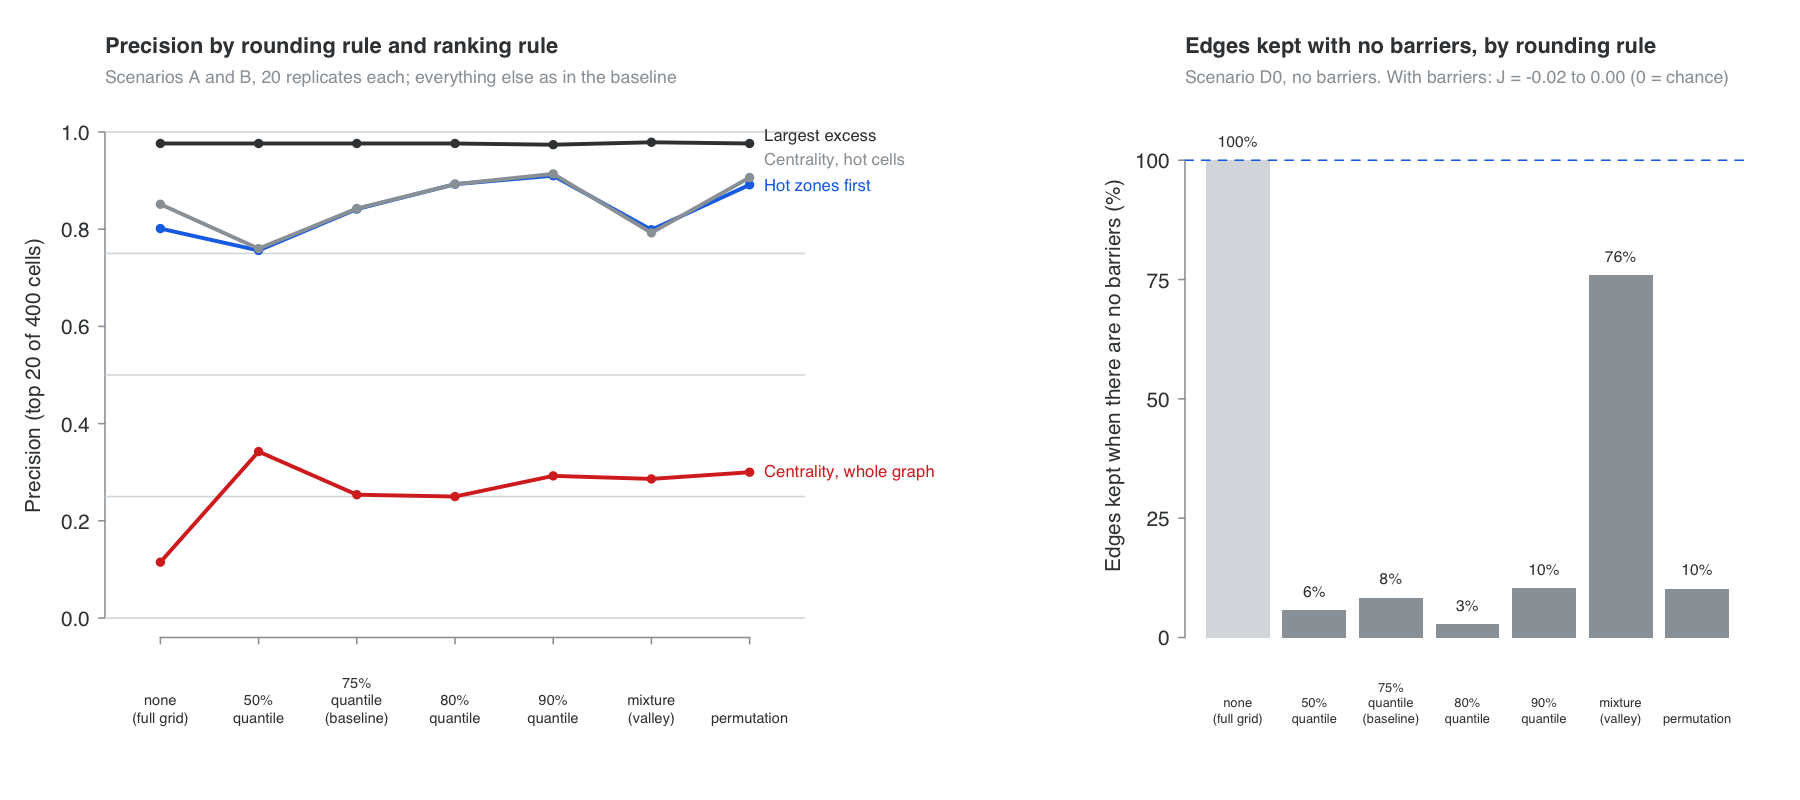
\includegraphics[width=\textwidth]{fig4_rounding_rules}
\caption{Left: precision of the top 20 of 400 cells by rounding rule and ranking rule (scenarios A and B pooled, 20 replicates each). Right: share of edges kept in scenario D0, where no edge should be removed. Rules: none (full grid), q50--q90 (quantile of the positive $b_{ij}$; q75 is the baseline), mix (two-component mixture), perm (permutation).}
\label{fig:app-rounding}
\end{figure}

\paragraph{Fine grid with weak clusters.}
On a $40\times40$ grid (cell side 25) with 50 or 200 points per cluster, scenario B, budget of 80 cells, 10 replicates, the rankings that use hot cells and connectivity reached, with no rounding, a precision of 0.44--0.48 (50 points) and 0.81--0.89 (200 points), against 0.29 and 0.80 for top residuals on the log scale. Rounding reduced the precision of hot zones first by 0.24 and 0.25 (75\% quantile), 0.18 and 0.17 (90\% quantile) and 0.06 and 0.10 (permutation) (Fig.~\ref{fig:app-finegrid}).

\begin{figure}[ht]
\centering
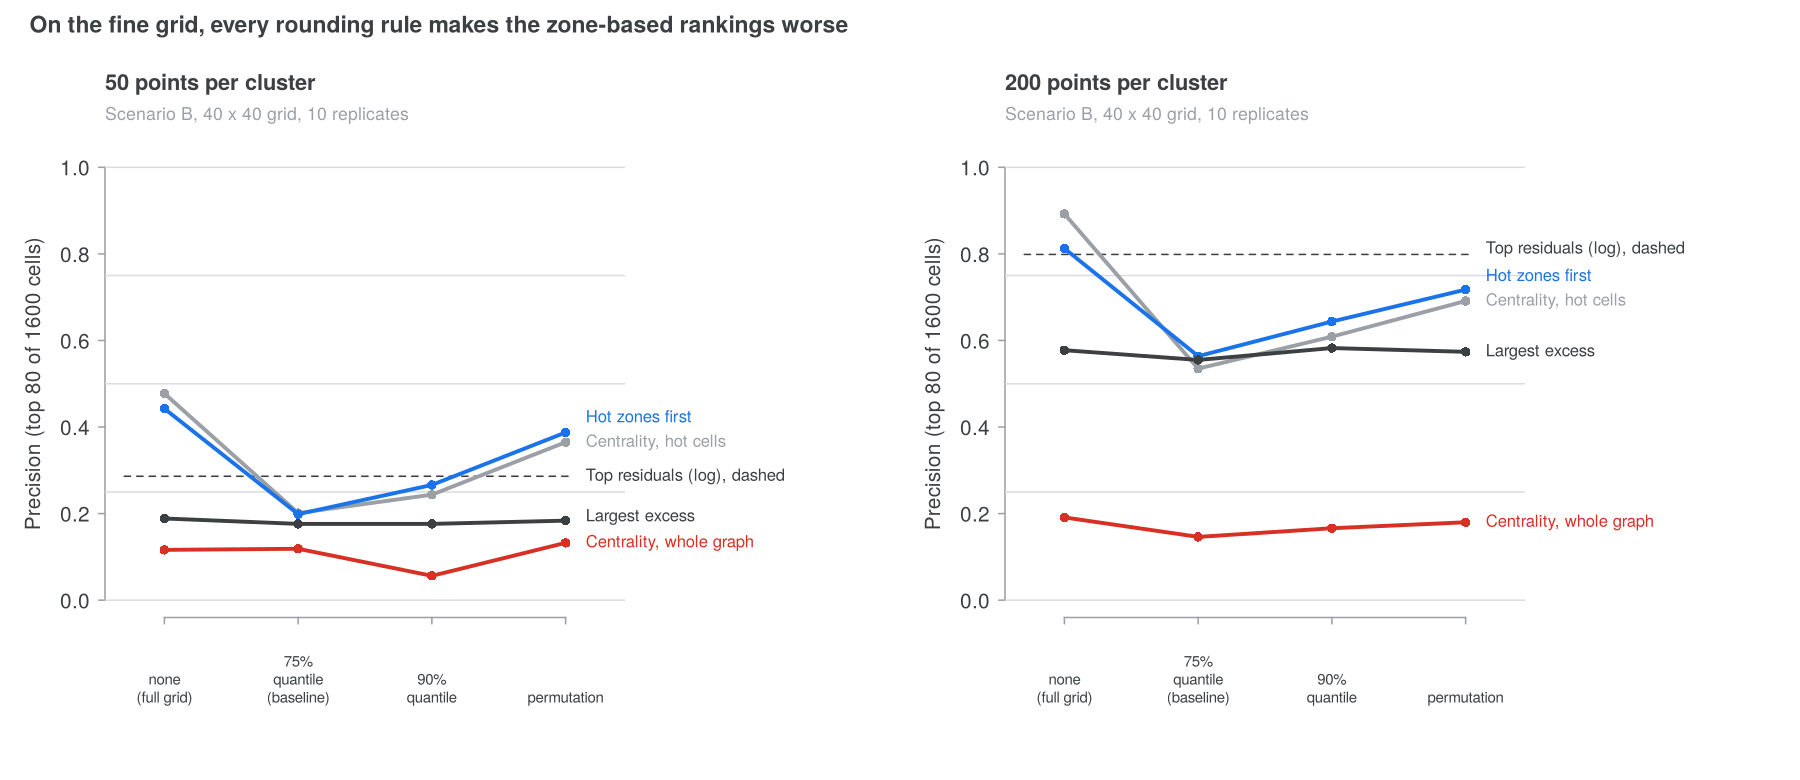
\includegraphics[width=\textwidth]{fig5_fine_grid}
\caption{Precision of the top 80 of 1600 cells by rounding rule and ranking rule on a $40\times40$ grid (scenario B, 10 replicates per panel). Dashed line: top residuals of $\log(Y+1)$ on $Z$. Rule labels as in Figure~\ref{fig:app-rounding}.}
\label{fig:app-finegrid}
\end{figure}

\paragraph{Recovery of a known graph.}
In scenario D, the AUC of $b_{ij}$ for separating real from barrier edges was 0.55, 0.55 and 0.45 for $\rho=0.5$, $0.8$ and $0.95$ with eigenvalue weights, and 0.55, 0.53 and 0.61 with squared coefficients $\hat\gamma_s^2$ as weights. The absolute difference between the residuals of neighbouring cells, $|e_i-e_j|$, gave 0.55, 0.65 and 0.96 (Fig.~\ref{fig:app-graph}). After the full procedure, Youden's $J$ ranged from $-0.02$ to $0.00$ across rounding rules. With 130--300 of 400 eigenvectors selected, $B$ differs from $A$ by a small number of patterns with global support, while a barrier is a local discontinuity.

\begin{figure}[ht]
\centering
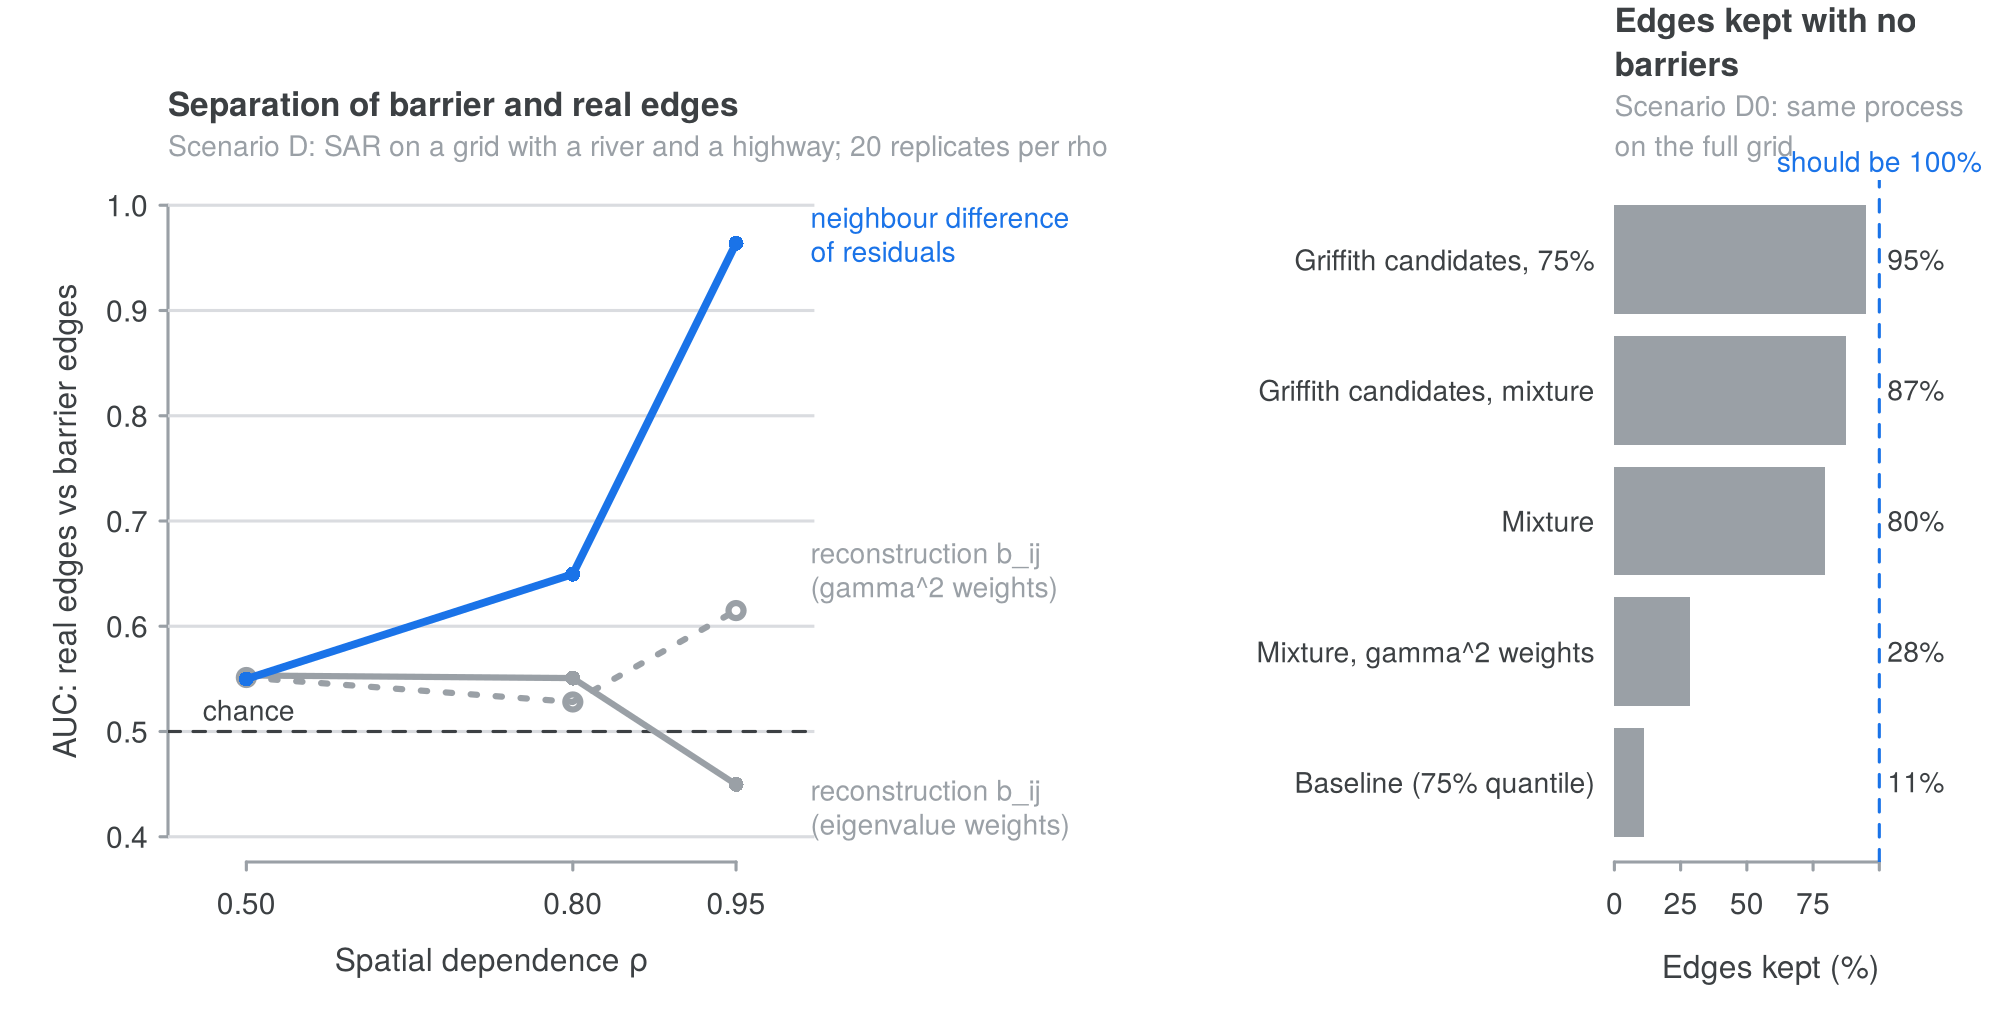
\includegraphics[width=\textwidth]{fig3_latent_graph}
\caption{Left: AUC for separating real edges from barrier edges in scenario D (20 replicates per $\rho$). Right: share of edges kept in scenario D0 by variant of the procedure.}
\label{fig:app-graph}
\end{figure}

\subsection{Conclusion}
\label{app:rec-conclusion}

In these simulations, no rounding rule increased the highest precision obtained without rounding by more than 0.01 (largest excess on the $20\times20$ grid; centrality among hot cells on the $40\times40$ grid). The reconstructed weights did not identify the edges removed by barriers, and most rounding rules removed most edges when no barrier was present. Ranking by centrality on the whole reconstructed graph selected cold cells in about half of the positions. The proposed procedure therefore uses the ESF step once, to estimate the spatial component $\hat f$ conditional on the covariates, and derives hot and cold zones from it on the contiguity graph $A$.

\end{appendices}

\end{document}
